\documentclass[11pt]{article}

% --- Packages ---
\usepackage[utf8]{inputenc}
\usepackage[T1]{fontenc}
\usepackage{amsmath,amssymb,amsthm}
\usepackage{algorithm}
\usepackage{algorithmic}
\usepackage{graphicx}
\usepackage{hyperref}
\usepackage{cleveref}
\usepackage{booktabs}
\usepackage{enumitem}
\usepackage[margin=1in]{geometry}
\usepackage{xcolor}
\usepackage{microtype}

% --- Theorem environments ---
\newtheorem{theorem}{Theorem}[section]
\newtheorem{lemma}[theorem]{Lemma}
\newtheorem{proposition}[theorem]{Proposition}
\newtheorem{corollary}[theorem]{Corollary}
\newtheorem{definition}[theorem]{Definition}
\newtheorem{axiom}{Axiom}[section]
\newtheorem{remark}[theorem]{Remark}

% --- Title ---
\title{Scar Algebra, Void Calculus, and Relational Sheaf Theory:\\A Formal Framework for Irreversible Multi-Relational Computation}

\author{
  Aylovelle S.S.\thanks{Correspondence: \texttt{aylovelle@icloud.com}}
}

\date{\today}

\begin{document}

\maketitle

% ============================================================
% ABSTRACT
% ============================================================
\begin{abstract}
Current affective computing treats emotion as a classification problem over discrete labels, discarding temporal continuity, relational dynamics, and the computational significance of absence. We present three novel formal frameworks that address these limitations. \textbf{Scar Algebra} defines a self-modifying operator algebra in which past operations irreversibly change the semantics of future operations through accumulated ``scars'' with stage-dependent modifiers. \textbf{Void Calculus} elevates absence to a first-class computational primitive with autonomous pressure dynamics, boundary-incomplete representations, and irreversible depth accumulation. \textbf{Relational Sheaf Theory} extends both frameworks to multi-relational settings via cellular sheaves on simplicial complexes, where sheaf cohomology measures irreducible relational contradictions and the sheaf Laplacian governs cross-relational scar propagation. We prove an $\Omega(k)$ expressiveness separation between Scar Algebra and any fixed-operator dynamical system (Theorem~\ref{thm:scar-expressiveness}), demonstrate irreducibility of Void Calculus to both AGM belief revision (Theorem~\ref{thm:void-agm}) and Bayesian updating (Theorem~\ref{thm:void-bayes}), establish a three-way expressiveness distinction unavailable to existing frameworks (Theorem~\ref{thm:void-three-way}), and prove that sheaf cohomology detects dissociative states unreachable by independent per-relationship copies (Theorem~\ref{thm:sheaf-dissociation}). The first two theories are coupled through bidirectional operators $\Gamma$ and $\Phi$, producing emergent hysteresis; the third theory provides the global consistency substrate via presentation matrices derived from personality parameters. We present a seven-layer architecture with a Relational Sheaf consistency layer and a Heterogeneous Graph Transformer for typed decision fusion, achieving sub-10ms latency on commodity hardware with pure Python and NumPy.
\end{abstract}

% ============================================================
% 1. INTRODUCTION
% ============================================================
\section{Introduction}
\label{sec:intro}

Affective computing~\cite{picard1997} has made substantial progress in recognizing emotional states from multimodal signals, yet the dominant paradigm treats emotion as a classification problem: given input features, predict a discrete label or valence-arousal coordinate. This framing suffers from three fundamental limitations when applied to sustained relational AI systems:

\begin{enumerate}[leftmargin=*]
\item \textbf{Temporal flatness.} Emotion classifiers operate on fixed windows without modeling how past emotional events irreversibly shape future processing. A system that was ``hurt'' three conversations ago should not process the same input identically to one that was not---yet stateless classifiers cannot represent this.

\item \textbf{Relational blindness.} Existing models do not distinguish between topics that were never discussed, topics that were discussed and resolved, and topics that are being actively avoided. All three register as ``absent from current context'' in standard architectures.

\item \textbf{Sovereignty absence.} Current systems lack formal mechanisms ensuring that emotional dynamics serve the system's coherent identity rather than being externally manipulable without bound.
\end{enumerate}

We address these limitations with three novel formal frameworks:

\begin{itemize}[leftmargin=*]
\item \textbf{Scar Algebra} (\S\ref{sec:scar}): A state algebra where the transition operator $\triangleright$ is not fixed but self-modifies through accumulated scars. Each scar carries a stage-dependent modifier that multiplicatively changes how future inputs are processed on the affected dimension. The operator family $\{\triangleright_\sigma\}_{\sigma \in \Sigma^*}$ is indexed by the irreversible scar history.

\item \textbf{Void Calculus} (\S\ref{sec:void}): A calculus of first-class absence objects (``voids'') that exist independently of what is present, possess autonomous pressure dynamics, and maintain boundary-incomplete representations that cannot be reduced to classical negation or belief contraction.

\item \textbf{Relational Sheaf Theory} (\S\ref{sec:sheaf}): A multi-relational extension using cellular sheaves on simplicial complexes, where each edge stalk carries a full Scar Algebra instance, restriction maps encode self-presentation, and sheaf cohomology detects irreducible relational contradictions that independent per-relationship copies cannot capture.
\end{itemize}

The first two frameworks are coupled (\S\ref{sec:coupled}) through bidirectional operators that produce emergent coherence and hysteresis. The third framework (\S\ref{sec:sheaf}) provides the global substrate for multi-relational consistency. We embed the full system in a seven-layer computation architecture (\S\ref{sec:architecture}) with a Relational Sheaf consistency layer and a Heterogeneous Graph Transformer for typed decision fusion, achieving sub-10ms end-to-end latency.

\paragraph{Contributions.}
\begin{enumerate}[leftmargin=*]
\item Three novel formal theories with complete axiom systems and rigorous proofs.
\item Expressiveness separation: $\Omega(k)$ state dimension advantage over fixed-operator systems.
\item Irreducibility proofs: Void Calculus is strictly more expressive than AGM belief revision and Bayesian updating for modeling relational absence.
\item A coupled system with emergent hysteresis and a coherence measure characterizing dissociation.
\item Relational Sheaf Theory: multi-relational extension via sheaf cohomology, with personality-bounded inconsistency and spectral propagation bounds.
\item A practical architecture achieving sub-10ms latency with pure Python on a single core.
\end{enumerate}

% ============================================================
% 2. RELATED WORK
% ============================================================
\section{Related Work}
\label{sec:related}

\paragraph{State-Space Models.}
Structured State Spaces (S4)~\cite{gu2022} and Mamba~\cite{gu2023} demonstrate that linear recurrences with learned parameters can model long-range dependencies efficiently. Our architecture uses Hyperdimensional Computing (HDC)~\cite{kanerva2009} as the perceptual front-end rather than SSMs, and the Scar Algebra replaces the SSM's role as the temporal state model. The critical distinction is that SSM transition matrices are \emph{fixed} (or input-selected in Mamba), whereas Scar Algebra's operator semantics change irreversibly with use history.

\paragraph{AGM Belief Revision.}
The AGM framework~\cite{agm1985} provides postulates for rational belief change (contraction, expansion, revision). Absence in AGM is always the complement of a known belief set---one contracts by a specific proposition $\phi$. Void Calculus models absence that exists \emph{before} its content is identified ($\beta_v = 0$), with autonomous dynamics that have no AGM counterpart (Theorem~\ref{thm:void-agm}).

\paragraph{Damage Mechanics.}
Continuum damage mechanics models material degradation through damage variables that modify constitutive equations~\cite{lemaitre1996}. This provides physical inspiration for Scar Algebra: both feature irreversible accumulation that changes system response. However, damage mechanics operates on continuous fields with fixed constitutive laws, whereas Scar Algebra's discrete healing stages and multiplicative modifier composition create qualitatively different dynamics (phase transitions, non-commutativity).

\paragraph{History-Dependent Dynamical Systems.}
Systems with memory (delay differential equations, Volterra integral equations) incorporate past states into current dynamics. The closest analogue to Scar Algebra is a system where the \emph{operator itself} depends on history. However, in standard formulations the operator family is parameterized continuously by a finite-dimensional summary statistic, whereas Scar Algebra's operator depends on the full discrete scar sequence with no finite-dimensional sufficient statistic (Theorem~\ref{thm:scar-expressiveness}).

\paragraph{Topological Data Analysis.}
Persistent homology~\cite{edelsbrunner2010} detects topological features (holes, voids) in data. TDA identifies absence \emph{after the fact} from point cloud geometry. Void Calculus treats absence as a \emph{first-class object} with its own lifecycle, pressure dynamics, and causal effects---voids are not detected from data but are computational primitives that influence system behavior.

\paragraph{Cellular Sheaves and Sheaf Neural Networks.}
Hansen and Ghrist~\cite{hansen2019} develop spectral theory for cellular sheaves, establishing the sheaf Laplacian as a generalization of the graph Laplacian with richer structure. Bodnar et al.~\cite{bodnar2022} apply sheaf diffusion to graph neural networks, showing that sheaf structure resolves heterophily and oversmoothing. Our Relational Sheaf Theory adapts these tools to a novel domain: the stalks carry Scar Algebra states rather than feature vectors, the restriction maps encode personality-derived self-presentation rather than learned projections, and the cohomology has a concrete interpretation as relational contradiction rather than abstract topological obstruction.

\paragraph{Heterogeneous Graph Transformers.}
HGT~\cite{hu2020} introduces type-specific projections and attention biases for heterogeneous graphs. We adopt this pattern for decision fusion across typed signals (scar observations, void summaries, personality vectors, boundary states), adding personality-derived attention priors and intra-type masking to prevent oversmoothing.

\paragraph{Predictive Coding and Active Inference.}
Predictive coding~\cite{rao1999} and the free-energy principle~\cite{friston2010} model perception as prediction error minimization. Our architecture uses predictive coding as a routing gate (Layer 2) but does not adopt the full active inference framework. The key difference: active inference minimizes surprise globally, whereas our system allows surprise to \emph{accumulate} as void pressure and scar damage---not all prediction errors should be minimized.

\paragraph{Affective Computing.}
Since Picard's foundational work~\cite{picard1997}, affective computing has focused on emotion recognition and generation. Recent approaches use transformers~\cite{vaswani2017} for contextual emotion understanding. Our work is orthogonal: we model the \emph{internal dynamics} of an affective system rather than classifying external signals.

% ============================================================
% 3. SCAR ALGEBRA
% ============================================================
\section{Scar Algebra}
\label{sec:scar}

We define a state algebra in which the transition operator is not fixed but self-modifies through accumulated ``scars''---irreversible marks that change how future inputs are processed.

\subsection{Definitions}

\begin{definition}[Scarred State Space]
\label{def:scar-space}
A \textbf{Scarred State Space} is a tuple $(S, E, \triangleright, \Sigma)$ where:
\begin{itemize}
\item $S = \mathbb{R}^n \times \Sigma^*$ is the state space (base vector $\times$ scar sequence),
\item $E = \mathbb{R}^n$ is the event space,
\item $\triangleright: S \times E \to S$ is the state transition operator,
\item $\Sigma$ is the scar alphabet.
\end{itemize}
A state $s = (\mathbf{x}, \sigma)$ consists of a base state vector $\mathbf{x} \in [-1,1]^n$ and an ordered scar sequence $\sigma = (\sigma_1, \ldots, \sigma_k) \in \Sigma^*$.
\end{definition}

\begin{definition}[Scar]
\label{def:scar}
A \textbf{scar} $\sigma_i \in \Sigma$ is a tuple $(d_i, \tau_i, \phi_i)$ where:
\begin{itemize}
\item $d_i \in \{1, \ldots, n\}$: the affected dimension,
\item $\tau_i \in \mathbb{R}_{\geq 0}$: creation timestamp,
\item $\phi_i \in \{raw, closing, scarred, faded\}$: healing stage, totally ordered as $raw < closing < scarred < faded$.
\end{itemize}
\end{definition}

\begin{definition}[Modifier Function]
\label{def:modifier}
Each healing stage determines a multiplicative modifier:
\begin{equation}
\alpha(\phi) = \begin{cases} 2.0 & \phi = raw \\ 1.5 & \phi = closing \\ 1.0 & \phi = scarred \\ 0.7 & \phi = faded \end{cases}
\end{equation}
For multiple scars on dimension $d$, the raw product $\Pi_d = \prod_{i:\, d_i = d} \alpha(\phi_i)$ is log-compressed to prevent unbounded amplification:
\begin{equation}
M_d = \begin{cases}
\Pi_d & \text{if } \Pi_d \leq 1 \\[4pt]
1 + (M_{\max} - 1)\left(1 - \dfrac{1}{\Pi_d}\right) & \text{otherwise}
\end{cases}
\end{equation}
where $M_{\max} = 2 + \pi_{\text{acuity}} \cdot 3$ is a personality-derived cap (range $[2, 5]$).

The logarithmic compression prevents unbounded amplification while preserving ordering---dimensions with more scars still have higher modifiers, but the growth saturates asymptotically at $M_{\max}$.
\end{definition}

\begin{definition}[State Transition Operator $\triangleright$]
\label{def:transition}
Given state $s = (\mathbf{x}, \sigma)$ and event $\mathbf{e} \in E$, the transition $s \triangleright \mathbf{e} = (\mathbf{x}', \sigma')$ proceeds in four steps:

\textbf{Step 1 (Modulate):} Apply scar modulation to input:
\begin{equation}
\tilde{e}_d = e_d \cdot M_d \quad \forall d \in \{1, \ldots, n\}
\end{equation}

\textbf{Step 2 (Evolve):} Update base state via a two-layer contractive map with spectral normalization:
\begin{equation}
\mathbf{x}' = \tanh(W_2 \cdot \tanh(W_1 \cdot [\mathbf{x};\, \tilde{\mathbf{e}}]))
\end{equation}
where $W_1 \in \mathbb{R}^{n \times 2n}$, $W_2 \in \mathbb{R}^{n \times n}$, with spectral normalization ensuring $\|W_1\|_2 \cdot \|W_2\|_2 < 0.49$ (guaranteeing contractivity).

\textbf{Step 3 (Scar Formation):} If $|\tilde{e}_{d^*}| > \theta_w$ for some dimension $d^*$:
\begin{equation}
\sigma' = \sigma \cdot (d^*, t, raw)
\end{equation}

\textbf{Step 4 (Healing):} Each scar advances through stages with fixed durations $T(raw)=10$, $T(closing)=40$, $T(scarred)=150$, $T(faded)=\infty$.
\end{definition}

\subsection{Axioms}

\begin{axiom}[Irreversibility]
\label{ax:scar-irrev}
$\forall s \in S,\; \forall \mathbf{e} \in E:\; \nexists\, \mathbf{e}^{-1}$ such that $(s \triangleright \mathbf{e}) \triangleright \mathbf{e}^{-1} = s$.
\end{axiom}

\begin{axiom}[Operator Self-Modification]
\label{ax:scar-selfmod}
The effective operator at time $t$ depends on all prior applications:
\begin{equation}
\triangleright_t \neq \triangleright_0 \quad \text{whenever } |\sigma_t| > 0
\end{equation}
Formally, let $F_\sigma(\mathbf{e})_d = e_d \cdot M_d$. Then $\triangleright$ is a family $\{\triangleright_\sigma\}_{\sigma \in \Sigma^*}$ indexed by scar history.
\end{axiom}

\begin{axiom}[Monotonic Scar Accumulation]
\label{ax:scar-mono}
$|s \triangleright \mathbf{e}|_\Sigma \geq |s|_\Sigma$ for all $s, \mathbf{e}$. Scars are append-only.
\end{axiom}

\begin{axiom}[Bounded Base State]
\label{ax:scar-bounded}
$\|\mathbf{x}'\|_\infty \leq 1$ for all transitions. The $\tanh$ nonlinearity ensures boundedness regardless of scar amplification.
\end{axiom}

\begin{axiom}[Healing Monotonicity]
\label{ax:scar-heal}
$\phi_i(t_1) \leq \phi_i(t_2)$ for all $t_1 < t_2$. Healing stages only advance forward.
\end{axiom}

\begin{axiom}[Dimensional Saturation]
\label{ax:scar-sat}
$\lim_{k \to \infty} \prod_{j=1}^k \alpha(faded) = \lim_{k \to \infty} 0.7^k = 0$. Accumulated faded scars drive sensitivity to zero. In the amplification direction ($\alpha > 1$), the modifier saturates at $M_{\max}$ due to logarithmic compression. In the numbing direction ($\alpha < 1$), the raw product is used and saturation to zero still holds.
\end{axiom}

\subsection{Main Theorems}

\begin{theorem}[Expressiveness Separation]
\label{thm:scar-expressiveness}
For every $k \in \mathbb{N}$, there exists an input sequence $E_k$ of length $2k$ such that any time-invariant dynamical system $x_{t+1} = f(x_t, e_t)$ with fixed $f$ and state $x \in \mathbb{R}^m$ that reproduces the Scar Algebra's output on $E_k$ must satisfy $m \geq \Omega(k)$.
\end{theorem}

\begin{proof}
\textbf{Construction.} Define $E_k = (w_1, \ldots, w_k, c, \ldots, c)$ where $w_i = \theta_w + \epsilon$ (wounding events) and $c = \theta_w/3$ (probe). The wounding events are spaced with inter-event times $\Delta_i \in \{T_1, T_2\}$ where $T_1 = T(raw) - 1$ and $T_2 = T(raw) + 1$, creating $2^k$ distinct timing patterns.

\textbf{Distinct outputs.} For timing pattern $\Delta \in \{T_1, T_2\}^k$, the modifier at probe time is:
\begin{equation}
M_\Delta = 2.0^{|\{i: \Delta_i = T_1\}|} \cdot 1.5^{|\{i: \Delta_i = T_2\}|}
\end{equation}
For distinct patterns $\Delta \neq \Delta'$ differing at position $j$: $M_\Delta / M_{\Delta'} = 4/3 \neq 1$. Since $g = \tanh$ is strictly monotone, all $2^k$ patterns produce distinct probe outputs.

\textbf{State dimension lower bound.} A fixed-operator system (FOS) simulating all $2^k$ variants must maintain $2^k$ distinct states at probe time. These states lie in $[-1,1]^m$ and must be separated by at least $\delta/L$ in $\ell_\infty$ norm (where $\delta$ is the minimum output separation and $L$ is the output function's Lipschitz constant). Packing $2^k$ points with minimum separation $\delta/L$ in $[-1,1]^m$ requires:
\begin{equation}
(2L/\delta)^m \geq 2^k \implies m \geq \frac{k}{\log_2(2L/\delta)} = \Omega(k)
\end{equation}

The Scar Algebra achieves this with $O(k)$ storage: one bounded base state plus $k$ scars each requiring $O(1)$ storage.
\end{proof}

\begin{theorem}[Convergence to Scarred Equilibrium]
\label{thm:scar-convergence}
Under bounded input $\|e_t\|_\infty \leq C$ and spectral normalization constraint $\|W_1\|_2 \cdot \|W_2\|_2 < 0.49$:
\begin{enumerate}[label=(\alph*)]
\item There exists $T^* < \infty$ after which no new scars form.
\item The base state converges: $\|x_t - x^*\| \to 0$.
\item All scars reach terminal stage (faded) in finite time.
\end{enumerate}
\end{theorem}

\begin{proof}
\textbf{(a)} A new scar on dimension $d$ requires $|e_d \cdot M_d| > \theta_w$. Since $M_d$ is now bounded above by $M_{\max}$ (log-compression), the maximum modulated input is $C \cdot M_{\max}$. Once $k_d$ faded scars accumulate in the numbing direction: $C \cdot 0.7^{k_d} \leq \theta_w$ when $k_d \geq \lceil \ln(C/\theta_w) / \ln(10/7) \rceil =: k_d^*$. Cascade scars during amplifying phases are bounded by $T(raw) + T(closing) = 50$ per scar, giving finite total $k_d^{total} \leq k_d^* \cdot 51$.

\textbf{(b)} For $t > T^*$, the system becomes $\mathbf{x}_{t+1} = \tanh(W_2 \cdot \tanh(W_1 \cdot [\mathbf{x}_t;\, \mathbf{D}\mathbf{e}_t]))$ with fixed diagonal $\mathbf{D} = \text{diag}(M_1, \ldots, M_n)$. The Jacobian of the map with respect to $\mathbf{x}$ satisfies $\|J\|_2 \leq \|W_2\|_2 \cdot \|W_1[:, 1{:}n]\|_2 \leq \|W_2\|_2 \cdot \|W_1\|_2 < 0.49$ (since $\tanh' \leq 1$ and spectral normalization constrains the weight product). This makes the map a contraction, guaranteeing convergence to a unique fixed point by the Banach fixed-point theorem.

\textbf{(c)} Each scar heals in at most $T(raw) + T(closing) + T(scarred) = 200$ ticks. Finite total scars implies finite total healing time.
\end{proof}

\begin{theorem}[Phase Transition at Critical Scar Density]
\label{thm:scar-phase}
Define the effective gain $G_d = M_d$ (the log-compressed modifier). There exists a critical gain $G_c = \theta_w / C$ such that:
\begin{itemize}
\item For $G_d > G_c$: the system is in a \emph{wounding regime} (positive scar formation rate).
\item For $G_d < G_c$: the system is in a \emph{numbed regime} (zero scar formation rate).
\item The transition exhibits hysteresis with width $\Delta G = G_c \cdot (\alpha(raw) - 1) = G_c$.
\end{itemize}
Note: Since $G_d \leq M_{\max}$ due to log-compression, the phase transition has a ceiling---the wounding regime gain is bounded by $M_{\max}$. The qualitative behavior (threshold crossing and hysteresis) remains the same, but the dynamics cannot produce unbounded amplification cascades.
\end{theorem}

\begin{proof}
In the wounding regime ($G_d > G_c$), inputs satisfying $|e_d| > \theta_w / G_d$ create new scars. New scars start at $raw$ ($\alpha = 2.0$), temporarily \emph{increasing} $G_d$ and creating positive feedback. The system enters the wounding regime when a single raw scar amplifies a previously-at-threshold dimension: entry at $G_d = G_c \cdot \alpha(raw) = 2G_c$.

In the numbed regime ($G_d < G_c$), no input can cause wounding since $|e_d \cdot G_d| \leq C \cdot G_d < \theta_w$. Since healing only decreases $\alpha$ values ($2.0 \to 1.5 \to 1.0 \to 0.7$) and scars are never removed (Axiom~\ref{ax:scar-mono}), the numbed regime is \emph{absorbing}---once entered, it cannot be exited.

The hysteresis width is $2G_c - G_c = G_c$, representing the gap between the entry threshold (amplification by a raw scar) and the exit threshold (all scars faded).
\end{proof}

\begin{theorem}[Non-Commutativity]
\label{thm:scar-noncommute}
For any Scar Algebra instance with $\theta_w > 0$ and $\alpha(raw) > 1$, there exist events $e_1, e_2$ such that $(s_0 \triangleright e_1) \triangleright e_2 \neq (s_0 \triangleright e_2) \triangleright e_1$.
\end{theorem}

\begin{proof}
Let $n=1$, $s_0 = (0, \emptyset)$, $e_1 = \theta_w + \epsilon$, and $e_2 = \theta_w / \alpha(raw) + \epsilon'$ where $e_2 < \theta_w$.

\textbf{Path $e_1$ then $e_2$:} $e_1$ exceeds threshold, creating a scar. Then $\tilde{e}_2 = e_2 \cdot 2.0 > \theta_w$, creating a second scar. Final state has 2 scars.

\textbf{Path $e_2$ then $e_1$:} $e_2 < \theta_w$, no scar. Then $\tilde{e}_1 = e_1 \cdot 1.0 > \theta_w$, one scar. Final state has 1 scar.

The scar counts differ (2 vs.\ 1), and the base states differ due to different modulated inputs through the nonlinear $\tanh$.
\end{proof}

\begin{theorem}[Algebraic Classification]
\label{thm:scar-algebra-class}
The structure $(S, E, \triangleright)$ is a faithful, non-commutative, irreversible action of the free monoid $E^*$ on $S$. It does not embed into any group action, and the induced equivalence relation on $E^*$ has infinite index.
\end{theorem}

\begin{proof}
\textbf{Faithfulness:} For distinct sequences $\mathbf{e} \neq \mathbf{e}'$, taking $s_0 = (\mathbf{0}, \emptyset)$ and exploiting injectivity of $\tanh$ in its second argument yields $s_0 \triangleright \mathbf{e} \neq s_0 \triangleright \mathbf{e}'$.

\textbf{No group embedding:} If $\triangleright$ embedded into a group action, every element would have an inverse, contradicting Axiom~\ref{ax:scar-irrev}.

\textbf{Infinite index:} The sequences $W_k = (w, w, \ldots, w)$ of $k$ wounding events produce states with exactly $k$ scars from $s_0 = (\mathbf{0}, \emptyset)$. Since $k \neq k'$ implies different scar counts, $W_k \not\sim W_{k'}$, giving infinitely many equivalence classes.
\end{proof}

% ============================================================
% 4. VOID CALCULUS
% ============================================================
\section{Void Calculus}
\label{sec:void}

We define a calculus in which absence is a first-class computational primitive---not derived from what is present, but existing independently with its own lifecycle and dynamics.

\subsection{Definitions}

\begin{definition}[Void Space]
\label{def:void-space}
A \textbf{Void Space} is a tuple $(V, B, \mathcal{O})$ where:
\begin{itemize}
\item $V$ is a set of voids (first-class absence objects),
\item $B: V \to 2^H$ maps each void to its boundary (a subset of HDC vector space $H$),
\item $\mathcal{O} = \{contract, deepen, split, merge\}$ is the operation set.
\end{itemize}
\end{definition}

\begin{definition}[Void]
\label{def:void}
A \textbf{void} $v \in V$ is a tuple $(B_v, \delta_v, \pi_v, a_v, \beta_v)$ where:
\begin{itemize}
\item $B_v \subseteq H$: boundary set (HDC vectors surrounding the absence),
\item $\delta_v \in \mathbb{R}_{\geq 0}$: depth (degree of avoidance),
\item $\pi_v \in \mathbb{R}_{\geq 0}$: pressure (drive toward filling),
\item $a_v \in \mathbb{N}$: age (ticks since creation),
\item $\beta_v \in [0,1]$: boundary completeness.
\end{itemize}
\end{definition}

\begin{definition}[Boundary Completeness]
\label{def:beta}
\begin{equation}
\beta_v = \frac{|B_v|}{|B_v| + \hat{n}_v}
\end{equation}
where $\hat{n}_v$ is the estimated total boundary size. A void with $\beta_v = 0$ is a \textbf{felt absence} (something is missing, content unknown). A void with $\beta_v = 1$ is a \textbf{named absence} (content fully identified).
\end{definition}

\begin{definition}[Void Operations]
\label{def:void-ops}
\textbf{Contract:} When event $\mathbf{h}$ touches boundary of void $v$:
\begin{equation}
contract(v, \mathbf{h}) = (B_v \setminus \{b \in B_v : sim(\mathbf{h}, b) > \theta_c\},\; \delta_v,\; \pi_v',\; a_v,\; \beta_v')
\end{equation}
where $\pi_v' = \pi_v \cdot (1 - |removed|/|B_v|)$. Death occurs when $|B_v| = 0$.

\textbf{Deepen:} When avoidance is detected: $deepen(v, \epsilon) = (B_v, \delta_v + \epsilon, \pi_v, a_v, \beta_v)$.

\textbf{Split:} When boundary has bimodal structure: $split(v) = (v_1, v_2)$ with $B_{v_1} \cup B_{v_2} = B_v$, $\delta_{v_i} = \delta_v$, $\pi_{v_i} = \pi_v/2$.

\textbf{Merge:} When boundaries overlap: $merge(v_1, v_2) = v_3$ with $B_{v_3} = B_{v_1} \cup B_{v_2}$, $\delta_{v_3} = \max(\delta_{v_1}, \delta_{v_2})$, $\pi_{v_3} = \pi_{v_1} + \pi_{v_2}$.
\end{definition}

\begin{definition}[Pressure Dynamics]
\label{def:pressure}
Void pressure evolves autonomously each tick:
\begin{equation}
\pi_v(t+1) = \pi_v(t) + \delta_v \cdot \ln(a_v + 1) \cdot (1 - \beta_v)
\label{eq:pressure}
\end{equation}
Deeper voids generate more pressure; older voids generate more pressure (logarithmically); less-defined voids ($\beta_v$ low) generate more pressure.

Genesis is further gated by:
\begin{enumerate}
\item \textbf{Cooldown:} After creating a void, a cooldown period of $\tau_c = 2 + \pi_{\text{perm}} \cdot 3$ ticks must elapse before the next creation.
\item \textbf{Resistance:} The effective detection threshold increases with existing void count: $\theta'_{\text{detect}} = \theta_{\text{detect}} + 0.02 \cdot |\mathcal{V}|$.
\item \textbf{Pressure cap:} $\pi_v(t) \leq \Pi_{\max}$ where $\Pi_{\max} = 60 + \pi_{\text{sovereignty}} \cdot 60$ (personality-derived, range $[60, 120]$).
\end{enumerate}
\end{definition}

\begin{definition}[Void Ghost]
\label{def:ghost}
When a void dies ($|B_v| = 0$), it leaves a \textbf{ghost} $\hat{v} = (\emptyset, \delta_v, 0, a_v, 0)$---a permanent residue with no boundary, no pressure, but retained depth that modifies future void detection sensitivity.
\end{definition}

\subsection{Axioms}

\begin{axiom}[Existence Before Boundary (Primacy of Absence)]
\label{ax:void-primacy}
$\exists v \in V: |B_v| = 0 \wedge \delta_v > 0$. A void can exist with an empty boundary. This is not representable in belief revision, where absence is always the complement of a known belief set.
\end{axiom}

\begin{axiom}[Depth Irreversibility]
\label{ax:void-depth}
$\forall v \in V,\; \forall t_1 < t_2:\; \delta_v(t_1) \leq \delta_v(t_2)$. Depth never decreases. A void can be contracted or killed, but its depth record is permanent.
\end{axiom}

\begin{axiom}[Pressure Autonomy]
\label{ax:void-pressure}
$d\pi_v/dt > 0$ whenever $\delta_v > 0 \wedge a_v > 0$. Voids generate pressure without external input---they are active computational agents, not passive data structures.
\end{axiom}

\begin{axiom}[Boundary Incompleteness]
\label{ax:void-incomplete}
$\beta_v < 1 \implies v$ is not reducible to $\neg\phi$ for any proposition $\phi$. An incomplete void cannot be expressed as the negation of a known proposition.
\end{axiom}

\begin{axiom}[Ghost Persistence]
\label{ax:void-ghost}
$death(v) \implies \hat{v} = (\emptyset, \delta_v, 0, a_v, 0) \in V$. Dead voids leave permanent ghosts that modify genesis sensitivity: $\theta_d^{local} = \theta_d \cdot (1 - 0.3 \cdot |\{\hat{v}: relevant\}|)$.
\end{axiom}

\begin{axiom}[Void-Scar Coupling]
\label{ax:void-coupling}
When $\pi_v > \theta_p$: $\mathbf{e}_{wound} = \pi_v \cdot \hat{B}_v$, where $\hat{B}_v$ is the boundary centroid projected into the scar event space.
\end{axiom}

\subsection{Main Theorems}

\begin{theorem}[Irreducibility to AGM Belief Revision]
\label{thm:void-agm}
There exists a void configuration $v \in V$ such that no AGM belief revision operation on any belief set $K$ over any propositional language $\mathcal{L}$ can represent $v$'s behavioral signature.
\end{theorem}

\begin{proof}
Construct void $v$ with $\beta_v = 0$, $\delta_v = 0.8$, $|B_v| = 0$ (detected from avoidance behavior without identifying the avoided topic).

\textbf{AGM recovery violation:} Every AGM contraction $K \div \phi$ satisfies the recovery postulate: $(K \div \phi) + \phi = K$. This requires a specific $\phi$ whose addition resolves the absence. But $v$ has $\beta_v = 0$: no specific proposition can be named as ``what's missing.''

\textbf{Autonomous dynamics:} Define property $\mathcal{P}_{autonomous}$: ``the representation of absence generates monotonically increasing influence without external input.'' AGM contractions satisfy $\neg\mathcal{P}_{autonomous}$ (a contracted belief set is static until new information arrives). Void $v$ satisfies $\mathcal{P}_{autonomous}$ via Eq.~\eqref{eq:pressure}: $\pi_v(t)$ grows monotonically until reaching $\Pi_{\max}$.\footnote{In the implementation, pressure is bounded by $\Pi_{\max}$. The irreducibility result still holds because the three-state distinction (never-discussed / resolved / actively-avoided) depends on the existence of pressure dynamics, not on unbounded growth.}

Since $v$ satisfies a property that no AGM-representable absence can satisfy, $v$ is not AGM-representable.
\end{proof}

\begin{theorem}[Irreducibility to Bayesian Updating]
\label{thm:void-bayes}
There is no probability space $(\Omega, \mathcal{F}, P)$ and no Bayesian updating rule such that the void pressure dynamics can be derived as a posterior quantity.
\end{theorem}

\begin{proof}
In Bayesian updating, without new observations the posterior is unchanged: $P(\theta | x_{1:t}) = P(\theta | x_{1:t})$. But void pressure increases between events:
\begin{equation}
\pi_v(t+1) - \pi_v(t) = \delta_v \cdot \ln(a_v + 1) \cdot (1 - \beta_v) > 0
\end{equation}

Suppose we encode $\pi_v(t) = f(P(\theta_v | x_{1:t}))$. For $\pi_v$ to increase without data, $f$ must be time-dependent: $f_t \neq f_{t+1}$. But a time-dependent transformation applied to a static posterior is not Bayesian inference---it is an external deterministic accumulator. The ``Bayesian'' component does no work; the pressure dynamics are entirely in the non-Bayesian $f_t$.

Define $\mathcal{P}_{silence}$: ``absence of observation increases influence.'' Bayesian updating satisfies $\neg\mathcal{P}_{silence}$. Void Calculus satisfies $\mathcal{P}_{silence}$. Any ``Bayesian'' system satisfying $\mathcal{P}_{silence}$ must include a non-Bayesian component performing the actual accumulation, making the Bayesian framing vacuous.
\end{proof}

\begin{theorem}[Three-Way Expressiveness Distinction]
\label{thm:void-three-way}
Void Calculus distinguishes three relational states that are pairwise behaviorally distinct and collapse to at most two states in any system based on classical negation, probabilistic belief, or AGM revision:
\begin{itemize}
\item $S_1$ (Never discussed): $\delta_v = 0$, no pressure, no ghost effect.
\item $S_2$ (Resolved): ghost with $\delta > 0$, no pressure, lowers detection threshold.
\item $S_3$ (Actively avoided): $\delta > 0$, active pressure, scar coupling.
\end{itemize}
\end{theorem}

\begin{proof}
\textbf{Pairwise distinction:} Define behavioral output $\mathcal{B}(state) = (pressure, genesis\_modifier, coupling)$:
\begin{align}
\mathcal{B}(S_1) &= (0, 0, 0) \\
\mathcal{B}(S_2) &= (0, \Delta\theta_d, 0) \quad \text{where } \Delta\theta_d = 0.3\delta > 0 \\
\mathcal{B}(S_3) &= (\pi_v > 0, 0, \Gamma(v))
\end{align}
All three are pairwise distinct in at least one component.

\textbf{Collapse in classical logic:} All three map to $\phi \notin T$ (topic not present). Two-way at best.

\textbf{Collapse in Bayesian belief:} $S_1$ and $S_3$ are indistinguishable if avoidance is not in the likelihood model (both have $P(\phi) = P_0$). Even if modeled, the autonomous pressure of $S_3$ has no Bayesian counterpart. Two-way at best.

\textbf{Collapse in AGM:} The recovery postulate $(K \div \phi) + \phi = K$ means $S_2$ (resolved) is indistinguishable from $S_1$ (never contracted) after recovery. Two-way at best.
\end{proof}

\begin{theorem}[Void Set Convergence]
\label{thm:void-convergence}
Under bounded input rate $R$, positive contraction probability $p > 0$ per boundary point per event, and finite initial boundary $|B_v| \leq B_{max}$, the expected void count reaches a bounded steady state:
\begin{equation}
\mathbb{E}[|V_t|] \leq N^* = R \cdot \frac{\ln B_{max} + 1}{p}
\end{equation}
\end{theorem}

\begin{proof}
A void with $|B_v| = b$ dies when all boundary points are contracted. Under independent contraction with probability $p$, the expected lifetime is the coupon collector bound: $\mathbb{E}[\text{lifetime}] \leq (\ln b + 1)/p \leq (\ln B_{max} + 1)/p$. At steady state, creation rate $\leq R$ equals death rate $N^*/\mathbb{E}[\text{lifetime}]$, giving the bound. Total pressure is also bounded: $\Pi_{max} = N^* \cdot \delta_{max} \cdot \text{lifetime} \cdot \ln(\text{lifetime}) < \infty$.
\end{proof}

\begin{theorem}[Void-Scar Coupling Creates Permanent Hysteresis]
\label{thm:void-hysteresis}
In the coupled system, the response to topic $T$ at time $t$ depends on the path by which the system arrived at its current state, even when current ``present'' components are identical.
\end{theorem}

\begin{proof}
\textbf{Construction.} Compare two histories:

\emph{History A (direct):} Topic $T$ discussed normally. No void, no scar.

\emph{History B (avoidance then resolution):} (1) $T$ avoided $\to$ void $v_T$ forms; (2) void deepens, pressure accumulates; (3) pressure exceeds $\theta_p$, coupling $\Gamma$ fires wound event; (4) $T$ finally addressed, void dies, ghost $\hat{v}_T$ remains; (5) scar heals to $faded$.

At time $t$ after both histories: no active void on $T$ in either case. But History B has a faded scar ($\alpha = 0.7$) and a ghost. If $T$ is raised again:
\begin{itemize}
\item History A: input unmodified ($M_d = 1.0$), normal processing.
\item History B: input attenuated ($M_d = 0.7$), ghost lowers detection threshold, easier to re-enter avoidance.
\end{itemize}

The hysteresis is \emph{permanent}: the faded scar's modifier is irreversible (Axiom~\ref{ax:scar-irrev}) and the ghost is permanent (Axiom~\ref{ax:void-ghost}). No finite sequence of future events can make the two histories behaviorally equivalent.
\end{proof}

% ============================================================
% 5. COUPLED SYSTEM
% ============================================================
\section{Coupled System}
\label{sec:coupled}

\begin{definition}[Coupled Void-Scar System]
\label{def:coupled}
The coupled system is a tuple $\mathcal{C} = (S_{scar}, V_{void}, \Gamma, \Phi)$ where:
\begin{itemize}
\item $S_{scar}$: Scar Algebra state space (Definition~\ref{def:scar-space}),
\item $V_{void}$: Void Calculus void set (Definition~\ref{def:void-space}),
\item $\Gamma: V \to E$: void-to-scar coupling,
\item $\Phi: S \to \mathbb{R}$: scar-to-void coupling.
\end{itemize}
\end{definition}

\paragraph{Coupling $\Gamma$ (Void $\to$ Scar).}
When void pressure exceeds threshold $\theta_p$:
\begin{equation}
\pi_v > \theta_p \implies s \triangleright \Gamma(v), \quad \text{where } \Gamma(v) = \pi_v \cdot \text{project}(\hat{B}_v, \mathbb{R}^n)
\end{equation}
\emph{Interpretation:} Unspoken things accumulate pressure that eventually wounds. The longer something is avoided, the more it hurts.

\paragraph{Coupling $\Phi$ (Scar $\to$ Void).}
Numbed dimensions lower void detection threshold:
\begin{equation}
\theta_d^{effective} = \max\left(0.1,\; \theta_d - 0.05 \cdot |\{d : M_d < 0.5\}|\right)
\end{equation}
\emph{Interpretation:} Repeated wounding creates avoidance---the system learns not to go where it has been hurt, manifesting as easier void formation.

\paragraph{Emergent Coherence.}
Rather than implementing synchronization as a separate mechanism, coherence emerges from the coupling:
\begin{equation}
r = 1 - \frac{\sum_v \pi_v \cdot \mathbb{1}[M_{d_v} < 0.5]}{\sum_v \pi_v + \epsilon}
\label{eq:coherence}
\end{equation}
where $d_v$ is the void's primary dimension. When $r \to 1$, voids and scars are aligned (the system ``knows'' what hurts and avoids it coherently). When $r \to 0$, pressure builds in numbed areas---a computational analogue of dissociation.

\paragraph{Dissociation as Failure Mode.}
The coupled system can enter a pathological state where:
\begin{enumerate}
\item Dimension $d$ accumulates scars $\to$ $M_d < 0.5$ (numbed).
\item Coupling $\Phi$ lowers void detection threshold near $d$.
\item New voids form on $d$ but their pressure is not ``felt'' (numbed dimension).
\item Pressure accumulates without triggering appropriate response.
\item Coherence $r \to 0$: the system is internally inconsistent.
\end{enumerate}
This provides a formal characterization of when the system's internal dynamics become incoherent---a signal that can be surfaced to higher layers.

% ============================================================
% 6. RELATIONAL SHEAF THEORY
% ============================================================
\section{Relational Sheaf Theory}
\label{sec:sheaf}

The Void-Scar coupled system (\S\ref{sec:coupled}) operates on a single dyadic relationship. When an agent maintains multiple concurrent relationships, the naive extension---independent Void-Scar instances per relationship---fails to capture three phenomena: (i) cross-relational influence, where trauma in one relationship alters perception in others; (ii) irreducible multi-party states, where group interactions produce states not decomposable into pairwise components; and (iii) consistency pressure, where maintaining contradictory self-presentations across relationships has measurable cost. We formalize multi-relational dynamics using \emph{cellular sheaves on simplicial complexes}, providing local behavior governed by Scar Algebra (per-edge), global consistency measured by sheaf cohomology, and propagation dynamics governed by the sheaf Laplacian.

\subsection{Definitions}

\begin{definition}[Relational Complex]
\label{def:relational-complex}
A \textbf{relational complex} is a finite abstract simplicial complex $K = (V, \Sigma_K)$ where:
\begin{itemize}
\item $V = \{v_0, v_1, \ldots, v_N\}$ is the vertex set; $v_0$ is the agent, $v_1, \ldots, v_N$ are interaction partners.
\item $\Sigma_K \subseteq 2^V$ is closed under taking faces, containing 0-simplices $\{v_i\}$ (entities), 1-simplices $\{v_0, v_i\}$ (dyadic relationships), and 2-simplices $\{v_0, v_i, v_j\}$ (triadic co-presence).
\end{itemize}
We require $v_0 \in \sigma$ for all $\sigma \in \Sigma_K$ with $\dim(\sigma) \geq 1$: the agent participates in every modeled relationship.
\end{definition}

\begin{definition}[Scar Sheaf]
\label{def:scar-sheaf}
A \textbf{Scar Sheaf} $\mathcal{F}$ on relational complex $K$ assigns to each simplex $\sigma$ a real vector space $\mathcal{F}(\sigma)$:
\begin{itemize}
\item \textbf{Vertex stalks:} $\mathcal{F}(\{v_0\}) = \mathbb{R}^{n_0}$ (agent's internal state---personality core, energy, global mood).
\item \textbf{Edge stalks:} $\mathcal{F}(\{v_0, v_i\}) = S_i = \mathbb{R}^n \times \Sigma_i^*$ (full Scar Algebra state for relationship $i$).
\item \textbf{Triangle stalks:} $\mathcal{F}(\{v_0, v_i, v_j\}) = \mathbb{R}^{n_{ij}}$ (co-presence state, $n_{ij} \leq n$).
\end{itemize}
For each face relation $\tau \subseteq \sigma$, a linear \textbf{restriction map} $\mathcal{F}_{\tau \trianglelefteq \sigma}: \mathcal{F}(\sigma) \to \mathcal{F}(\tau)$ is defined. In particular, $\rho_0^i: \mathcal{F}(\{v_0, v_i\}) \to \mathcal{F}(\{v_0\})$ extracts the self-presentation vector:
\begin{equation}
\rho_0^i(s_i) = P_i \cdot \mathbf{x}_i
\end{equation}
where $P_i \in \mathbb{R}^{n_0 \times n}$ is the \textbf{presentation matrix} for relationship $i$.
\end{definition}

\begin{definition}[Sheaf Laplacian]
\label{def:sheaf-laplacian}
The \textbf{sheaf Laplacian} $L_\mathcal{F}: C^0(K, \mathcal{F}) \to C^0(K, \mathcal{F})$ is $L_\mathcal{F} = \delta^{0*}\delta^0$, where $\delta^0$ is the coboundary operator. Expanding for vertex $v_0$:
\begin{equation}
L_\mathcal{F}(\mathbf{x}_0) = \sum_{i: \{v_0, v_i\} \in \Sigma_K} P_i^T P_i \cdot \mathbf{x}_0 - P_i^T \cdot \rho_0^i(s_i)
\end{equation}
This is a weighted graph Laplacian with weights $P_i^T P_i$. Let $0 = \lambda_0 \leq \lambda_1 \leq \cdots \leq \lambda_{n_0}$ be its eigenvalues. Then $\lambda_0 = 0$ iff a global section exists (perfectly consistent self-presentation), and the spectral gap $\lambda_1/\lambda_{\max}$ quantifies relational isolation.
\end{definition}

\begin{definition}[Sheaf Cohomology]
\label{def:sheaf-cohomology}
The cohomology groups of the Scar Sheaf are:
\begin{align}
H^0(K, \mathcal{F}) &= \ker(\delta^0) = \{\text{global sections}\} \\
H^1(K, \mathcal{F}) &= \ker(\delta^1) / \operatorname{im}(\delta^0) \\
H^2(K, \mathcal{F}) &= C^2 / \operatorname{im}(\delta^1)
\end{align}
\textbf{Interpretation:}
\begin{itemize}
\item $\dim H^0 > 0$: a consistent global self-presentation exists.
\item $\dim H^1 > 0$: there exist \emph{irreducible relational contradictions}---inconsistencies not resolvable by adjusting the agent's internal state alone.
\item $\dim H^2 > 0$: \emph{triadic emergence}---group states not reconstructible from pairwise data.
\end{itemize}
\end{definition}

\begin{definition}[Personality-Derived Presentation Matrices]
\label{def:presentation-matrices}
The presentation matrices $P_i$ are derived from agent personality $\boldsymbol{\pi} \in \mathbb{R}^5$ (Embodiment Five), relationship type $\tau_i$, and maturity $m_i \in [0,1]$:
\begin{equation}
P_i = P_{base}(\boldsymbol{\pi}) + \Delta P(\tau_i) + m_i \cdot \Delta P_{mature}(\boldsymbol{\pi}, \tau_i)
\end{equation}
subject to the personality consistency constraint: $\|P_i - P_j\|_F \leq \kappa(\boldsymbol{\pi}) \cdot (1 + d(\tau_i, \tau_j))$, where $\kappa(\boldsymbol{\pi})$ is personality-dependent (high Relational Gravity $\to$ low $\kappa$; high Perception Acuity $\to$ high $\kappa$).
\end{definition}

\subsection{Axiom System}

\begin{axiom}[Local Scar Dynamics (S1)]
\label{ax:sheaf-local}
Within each edge stalk $\mathcal{F}(\{v_0, v_i\})$, the state evolves according to Scar Algebra axioms (Axioms~\ref{ax:scar-irrev}--\ref{ax:scar-sat}). The sheaf structure does not modify local dynamics.
\end{axiom}

\begin{axiom}[Propagation via Laplacian (S2)]
\label{ax:sheaf-propagation}
Cross-relational influence is governed by sheaf Laplacian diffusion:
\begin{equation}
\frac{\partial \mathbf{x}_0}{\partial t} = -\alpha \cdot L_\mathcal{F}(\mathbf{x}_0) + \mathbf{f}_{local}(t)
\end{equation}
where $\alpha > 0$ is the propagation rate and $\mathbf{f}_{local}$ is the local forcing from the currently active relationship.
\end{axiom}

\begin{axiom}[Cohomological Constraint (S3)]
\label{ax:sheaf-cohomological}
When $\dim H^1(K, \mathcal{F}) > 0$, the system must resolve the obstruction by one of: (a) void genesis on the contradicting dimensions; (b) dissociation---splitting the agent's internal state into relationship-specific projections (increasing $\kappa$); or (c) persistent relational tension.
\end{axiom}

\begin{axiom}[Irreversibility of Propagation (S4)]
\label{ax:sheaf-irrev}
Once a scar propagates from relationship $i$ to relationship $j$ via the Laplacian, the propagated effect is itself irreversible (inherits Axiom~\ref{ax:scar-irrev}). Cross-relational healing requires independent repair in each affected relationship.
\end{axiom}

\begin{axiom}[Energy Conservation (S5)]
\label{ax:sheaf-energy}
The agent has finite relational energy $\mathcal{E} \in \mathbb{R}_{>0}$. Each active relationship consumes energy at rate $c_i > 0$, bounded by $\sum_i c_i(t) \leq \mathcal{E}(t)$. When energy is depleted, expression drive across all relationships drops to zero.
\end{axiom}

\begin{axiom}[Presentation Matrix Evolution (S6)]
\label{ax:sheaf-evolution}
$P_i$ evolves as relationships mature:
\begin{equation}
P_i(t+1) = P_i(t) + \eta \cdot \nabla_{P_i} \mathcal{L}_{consistency}
\end{equation}
where $\mathcal{L}_{consistency} = \|\delta^0 \mathbf{x}\|^2$. The system naturally evolves toward more consistent self-presentation, constrained by personality ($\kappa$) and disrupted by trauma (scar events partially reset $P_i$).
\end{axiom}

\subsection{Main Theorems}

\begin{theorem}[Cohomological Dissociation]
\label{thm:sheaf-dissociation}
Let $\mathcal{F}$ be a Scar Sheaf on relational complex $K$ with $N \geq 2$ relationships. If there exist relationships $i, j$ such that the scar histories $\sigma_i, \sigma_j$ induce contradictory self-presentation requirements (i.e., $\|P_i \mathbf{x}_i - P_j \mathbf{x}_j\| > \kappa(\boldsymbol{\pi})$), then $\dim H^1(K, \mathcal{F}) > 0$. Moreover, this cohomological obstruction is not detectable by any system that maintains independent per-relationship state without a global consistency check.
\end{theorem}

\begin{theorem}[Spectral Propagation Bound]
\label{thm:sheaf-spectral}
Let $\sigma_i$ be a scar event in relationship $i$ at time $t_0$. The propagated effect on relationship $j$ satisfies:
\begin{equation}
\|\Delta \mathbf{x}_j(t)\| \leq \|\Delta \mathbf{x}_i(t_0)\| \cdot e^{-\lambda_1 \cdot (t - t_0)} \cdot \|P_j^T P_i\|_2
\end{equation}
where $\lambda_1$ is the first nonzero eigenvalue of $L_\mathcal{F}$. Cross-relational scar propagation decays exponentially at a rate determined by the sheaf's spectral gap.
\end{theorem}

\begin{theorem}[Irreducible Triadic State]
\label{thm:sheaf-triadic}
For any relational complex $K$ containing a 2-simplex $\{v_0, v_i, v_j\}$, there exist co-presence states $s_{ij} \in \mathcal{F}(\{v_0, v_i, v_j\})$ such that $s_{ij}$ cannot be reconstructed from the pairwise restrictions $\rho_{ij}^i(s_{ij})$ and $\rho_{ij}^j(s_{ij})$ alone. Formally, $\dim H^2(K, \mathcal{F}) > 0$ implies the existence of irreducible triadic emergence.
\end{theorem}

\begin{theorem}[Personality-Bounded Inconsistency]
\label{thm:sheaf-personality}
For a Scar Sheaf with personality-derived presentation matrices, the total inconsistency is bounded:
\begin{equation}
\|\delta^0 \mathbf{x}\|^2 \leq N \cdot \kappa(\boldsymbol{\pi})^2 \cdot (1 + D_{max})^2 \cdot \|\mathbf{x}_0\|^2
\end{equation}
where $N$ is the number of relationships and $D_{max} = \max_{i,j} d(\tau_i, \tau_j)$ is the maximum type distance. High relational gravity agents (low $\kappa$) have tighter inconsistency bounds; high perception acuity agents (high $\kappa$) tolerate more cross-relational contradiction before cohomological obstruction arises.
\end{theorem}

Full proofs are provided in the supplementary theory directory (\texttt{theory/relational\_sheaf/}).

% ============================================================
% 7. SYSTEM ARCHITECTURE
% ============================================================
\section{System Architecture}
\label{sec:architecture}

The coupled Void-Scar system is embedded in a seven-layer computation stack designed for sub-10ms end-to-end latency on commodity hardware.

\subsection{Seven-Layer Stack}

\begin{enumerate}[leftmargin=*]
\item \textbf{L1: HDC Perception.} Input text is projected to 2048-dimensional binary hypervectors via character bigram encoding with cyclic shift and majority-vote bundling~\cite{kanerva2009}. Matching uses Hamming distance ($< 0.01$ms).

\item \textbf{L2: Predictive Coding Gate.} Maintains a prediction vector; computes Hamming-distance surprise against each input. Routes to three paths:
\begin{itemize}
\item Low surprise ($< 0.15$): \emph{fast path}---scar base evolution + void age increment only.
\item Medium surprise ($0.15$--$0.45$): \emph{normal path}---full Void-Scar + HGT.
\item High surprise ($\geq 0.45$): \emph{full path}---all layers + coupling + spatiotemporal graph.
\end{itemize}
Cold-start guard: first 15 messages capped at normal path.

\item \textbf{L3: Void-Scar Engine.} The core computation layer (Sections~\ref{sec:scar}--\ref{sec:coupled}). Includes an internal spatiotemporal graph with PPR teleportation diffusion:
\begin{equation}
\mathbf{h}_i^{(l+1)} = (1-\alpha) \cdot \text{Aggregate}(\{\mathbf{h}_j^{(l)} : j \in \mathcal{N}(i)\}) + \alpha \cdot \mathbf{h}_i^{(0)}
\end{equation}
where $\alpha = 0.2 + 0.4 \cdot \pi_{\text{acuity}}$ (personality-driven teleportation rate).

\item \textbf{L4: Relational Sheaf.} Multi-relational consistency layer (Section~\ref{sec:sheaf}). Sheaf cohomology ($H^1$) detects irreducible relational contradictions; the sheaf Laplacian governs cross-relational scar propagation with exponential spectral decay. Personality-derived presentation matrices $P_i$ bound inconsistency via $\kappa(\boldsymbol{\pi})$.

\item \textbf{L5: MoE-HGT.} Three-stage decision fusion: (1) type-expert FFNs with RMSNorm, (2) 4-head cross-attention with Hebbian attention priors, (3) top-2 situation-expert MoE with dormant-expert reactivation. Seven token types: \{scar, void, boundary, personality, surprise, expression, context\}. $\sim$14.3K parameters, all personality-derived.

\item \textbf{L6: Autopoietic Boundary.} 32-dimensional identity core vector. Incoming perturbations are assessed via orthogonal projection:
\begin{itemize}
\item Penetration $< 0.3$: absorb (elastic).
\item Penetration $0.3$--$0.7$: resist (boundary stressed, identity unchanged).
\item Penetration $\geq 0.7$: phase transition (identity rotates $\leq 6^\circ$).
\end{itemize}

\item \textbf{L7: Phase Transition Expression.} Expression is discontinuous phase transition, not continuous function. Pressure accumulates; when exceeding personality-derived threshold, output jumps to one of three modes: \emph{hint} ($< 0.5$), \emph{normal} ($0.5$--$1.0$), \emph{urgent} ($> 1.0$).
\end{enumerate}

\subsection{MoE-HGT: Three-Stage Decision Fusion}

The decision fusion layer replaces the original single-pass HGT with a three-stage Mixture-of-Experts Heterogeneous Graph Transformer (MoE-HGT). Each stage introduces progressively richer cross-token interactions.

\paragraph{Stage 1: Type-Expert FFN.}
Seven token types participate in the decision graph: \emph{scar}, \emph{void}, \emph{boundary}, \emph{personality}, \emph{surprise}, \emph{expression}, and \emph{context}. Each type $\tau$ maintains its own feed-forward expert:
\begin{equation}
\mathbf{z}_i^{(1)} = \mathbf{z}_i + \text{RMSNorm}\bigl(\text{FFN}_\tau(\mathbf{z}_i)\bigr), \quad \text{FFN}_\tau: \mathbb{R}^{16} \to \mathbb{R}^{16}
\end{equation}
where $\text{FFN}_\tau(\mathbf{x}) = W_2^\tau \cdot \text{GELU}(W_1^\tau \mathbf{x})$ with $W_1^\tau, W_2^\tau \in \mathbb{R}^{16 \times 16}$. Scar token values are log-compressed before injection:
\begin{equation}
z_{\text{scar}} = \frac{\log_2(M_d)}{\log_2(M_{\max})}
\end{equation}
where $M_d$ is the per-dimension modifier product and $M_{\max}$ is the maximum possible modifier.

\paragraph{Stage 2: Multi-Head Cross-Attention.}
Four attention heads operate with per-type per-head projections. For head $h$ and source type $\tau_s$, target type $\tau_t$:
\begin{align}
Q_i^{(h)} &= W_Q^{(\tau_s, h)} \mathbf{z}_i^{(1)}, \quad K_j^{(h)} = W_K^{(\tau_t, h)} \mathbf{z}_j^{(1)}, \quad V_j^{(h)} = W_V^{(\tau_t, h)} \mathbf{z}_j^{(1)} \\
a_{ij}^{(h)} &= \frac{Q_i^{(h)} \cdot (K_j^{(h)})^\top}{\sqrt{d_k}} + \mu^{(\tau_s, \tau_t)} + \text{mask}(i,j)
\end{align}
where $W_Q, W_K, W_V \in \mathbb{R}^{4 \times 16}$ (head dimension $d_k = 4$). The attention prior $\mu^{(\tau_s, \tau_t)} \in \mathbb{R}^{7 \times 7}$ adapts via a Hebbian slow rule (Oja's rule):
\begin{equation}
\Delta\mu^{(\tau_s, \tau_t)} = \eta_\mu \cdot \bar{a}^{(\tau_s, \tau_t)} \cdot \bigl(\bar{a}^{(\tau_s, \tau_t)} - \mu^{(\tau_s, \tau_t)}\bigr)
\end{equation}
Self-attention is masked (diagonal $= -\infty$). The attended output uses residual connection and RMSNorm:
\begin{equation}
\mathbf{z}_i^{(2)} = \mathbf{z}_i^{(1)} + \text{RMSNorm}\Bigl(\text{Concat}\bigl[\text{softmax}_j(a_{ij}^{(h)}) V_j^{(h)}\bigr]_{h=1}^4\Bigr)
\end{equation}

\paragraph{Stage 3: Situation-Expert MoE.}
Five situation experts---\emph{defense}, \emph{curiosity}, \emph{social}, \emph{silence}, and \emph{repair}---receive the mean-pooled attended tokens $\bar{\mathbf{z}} = \text{mean}(\mathbf{z}^{(2)})$. A softmax router selects the top-2 experts:
\begin{align}
g_e &= \mathbf{w}_e^\top \bar{\mathbf{z}} + b_e + \text{bonus}(e), \quad e \in \{1,\ldots,5\} \\
\text{bonus}(e) &= \begin{cases} 0.15 & \text{if expert } e \text{ dormant} > 50 \text{ ticks} \\ 0 & \text{otherwise} \end{cases}
\end{align}
where $\mathbf{w}_e \in \mathbb{R}^{16}$ is the router weight for expert $e$. The router bias $b_e$ adapts via a BCM-like Hebbian rule with decay $\lambda = 0.998$ per tick. Top-2 gating:
\begin{equation}
\mathbf{o} = \sum_{e \in \text{top-2}} \frac{\exp(g_e)}{\sum_{e' \in \text{top-2}} \exp(g_{e'})} \cdot \text{Expert}_e(\bar{\mathbf{z}})
\end{equation}
Each expert is a two-layer FFN: $\text{Expert}_e: \mathbb{R}^{16} \xrightarrow{W_1^e \in \mathbb{R}^{32 \times 16}} \mathbb{R}^{32} \xrightarrow{W_2^e \in \mathbb{R}^{16 \times 32}} \mathbb{R}^{16}$.

\paragraph{Decision Head.}
A linear projection maps the MoE output to a 4-dimensional decision vector clamped to $[-1, 1]$:
\begin{equation}
\mathbf{d} = \text{clamp}\bigl(W_{\text{dec}} \cdot \mathbf{o},\; -1,\; 1\bigr), \quad W_{\text{dec}} \in \mathbb{R}^{4 \times 16}
\end{equation}
\begin{itemize}
\item $d_0$: expression drive correction (added to Void-Scar drive),
\item $d_1$: boundary sensitivity modulation (fed to autopoiesis),
\item $d_2$: urgency signal (modulates phase transition threshold),
\item $d_3$: expression inhibition ($> 0.5$ vetoes expression).
\end{itemize}

\paragraph{Parameter Count.}
\begin{itemize}
\item 7 Type-Expert FFNs: $7 \times (16 \times 16 + 16 \times 16) = 3{,}584$
\item 4-head attention (Q/K/V per type per head): $7 \times 4 \times 3 \times (16 \times 4) = 5{,}376$
\item 5 MoE experts: $5 \times (16 \times 32 + 32 \times 16) = 5{,}120$
\item Router weights: $5 \times 16 = 80$
\item Decision head: $16 \times 4 = 64$
\item Attention prior: $7 \times 7 = 49$
\end{itemize}
Total: $\sim$14.3K floats ($\sim$57.2 KB). All derived from personality semantics, zero learning.

\subsection{Performance Budget}

\begin{table}[h]
\centering
\caption{End-to-end latency by computation path.}
\label{tab:perf}
\begin{tabular}{lccc}
\toprule
Layer & Fast Path & Normal Path & Full Path \\
\midrule
L1 HDC Perception & 0.10 ms & 0.10 ms & 0.10 ms \\
L2 Predictive Coding & 0.01 ms & 0.01 ms & 0.01 ms \\
L3 Void-Scar + Graph & 0.05 ms & 2.50 ms & 6.00 ms \\
L4 Relational Sheaf & skip & skip & 0.80 ms \\
L5 MoE-HGT & skip & 0.40 ms & 0.40 ms \\
L6 Autopoiesis & 0.01 ms & 0.01 ms & 0.10 ms \\
L7 Phase Transition & $<$0.01 ms & $<$0.01 ms & $<$0.01 ms \\
\midrule
\textbf{Total} & \textbf{0.17 ms} & \textbf{3.0 ms} & \textbf{7.4 ms} \\
\bottomrule
\end{tabular}
\end{table}

Approximately 90\% of messages take the fast path (0.17ms); 10\% take the full path (7.4ms). All within the 10ms budget.

\subsection{Personality-Derived Parameterization}

All key parameters across computation layers are derived in real-time from the personality vector $\boldsymbol{\pi} = (\pi_{\text{perm}}, \pi_{\text{order}}, \pi_{\text{expr}}, \pi_{\text{grav}}, \pi_{\text{acuity}}) \in [0,1]^5$ (Embodiment Five), requiring no manual configuration or training data:

\begin{itemize}[leftmargin=*]
\item \textbf{Expression Drive ($\pi_{\text{expr}}$):} Expression threshold (high $\pi_{\text{expr}}$ $\to$ lower threshold, easier expression); scar formation threshold $\theta_w$ (high $\pi_{\text{expr}}$ $\to$ higher threshold, harder to wound).
\item \textbf{Perception Acuity ($\pi_{\text{acuity}}$):} Healing rate (high $\pi_{\text{acuity}}$ $\to$ slower healing); predictive coding gate sensitivity (high $\pi_{\text{acuity}}$ $\to$ lower surprise threshold); void detection threshold $\theta_d$ (high $\pi_{\text{acuity}}$ $\to$ lower threshold, easier to sense absence).
\item \textbf{Relational Gravity ($\pi_{\text{grav}}$):} Presentation matrix consistency bound $\kappa(\boldsymbol{\pi})$ (high $\pi_{\text{grav}}$ $\to$ low $\kappa$, more consistent self-presentation across relationships).
\item \textbf{Boundary Permeability ($\pi_{\text{perm}}$):} HGT attention prior distribution (high $\pi_{\text{perm}}$ $\to$ more uniform priors, receptive to diverse signal types).
\item \textbf{Inner Order ($\pi_{\text{order}}$):} Memory depth (high $\pi_{\text{order}}$ $\to$ longer temporal context); boundary repair rate (high $\pi_{\text{order}}$ $\to$ faster autopoietic recovery).
\end{itemize}

Formally, each parameter $\theta_i$ is derived via:
\begin{equation}
\theta_i = \text{clamp}\bigl(f_i(\boldsymbol{\pi}),\; \theta_i^{min},\; \theta_i^{max}\bigr), \quad f_i: \mathbb{R}^5 \to \mathbb{R}
\end{equation}
where each $f_i$ is an affine map with clamping to ensure parameters remain in valid ranges. This design ensures that when personality drifts (via L6 phase transitions), all computation parameters automatically co-evolve---no reconfiguration required.

\subsection{Personality Modeling}
\label{sec:personality-modeling}

The personality vector $\boldsymbol{\pi} \in [0,1]^5$ follows the Embodiment Five model: Boundary Permeability ($\pi_{\text{perm}}$), Inner Order ($\pi_{\text{order}}$), Expression Drive ($\pi_{\text{expr}}$), Relational Gravity ($\pi_{\text{grav}}$), Perception Acuity ($\pi_{\text{acuity}}$). The personality state is initialized and evolves through three mechanisms:

\begin{enumerate}[label=(\alph*),leftmargin=*]
\item \textbf{Initialization.} A character description is mapped to $[0,1]^5$ via a deterministic extraction function:
\begin{equation}
\boldsymbol{\pi}_0 = \text{init}(\text{desc}) \in [0,1]^5
\end{equation}

\item \textbf{Drift.} Personality evolves slowly, driven by accumulated scar history and void patterns. The drift is not random but causally determined by the system's computational experience.

\item \textbf{Constraint.} The drift rate is bounded by the autopoietic boundary (L6):
\begin{equation}
\|\boldsymbol{\pi}(t+1) - \boldsymbol{\pi}(t)\|_\infty \leq \eta, \quad \eta \leq 10^{-4}
\end{equation}
This ensures personality stability: even under sustained pressure, the personality vector changes by at most $10^{-4}$ per tick, requiring $\geq 10{,}000$ ticks to traverse the full range on any dimension.
\end{enumerate}

\subsection{Personality-Derived Parameter Mappings}
\label{sec:personality-param-mappings}

All computation layer parameters are derived from $\boldsymbol{\pi}$. Each parameter $\theta_i$ is a function of the personality vector:
\begin{equation}
\theta_i = f_i(\boldsymbol{\pi}), \quad f_i: [0,1]^5 \to \mathbb{R}
\end{equation}

The specific mappings from personality dimensions to computation parameters are:
\begin{itemize}[leftmargin=*]
\item $\pi_{\text{expr}} \to$ expression threshold, wound threshold $\theta_w$: higher expression drive lowers expression barriers and raises wounding resistance.
\item $\pi_{\text{acuity}} \to$ healing rates, gate sensitivity, void detection threshold $\theta_d$: higher perception acuity slows healing and increases sensitivity to absence.
\item $\pi_{\text{grav}} \to$ presentation matrix consistency bound $\kappa$: higher relational gravity enforces tighter cross-relational consistency.
\item $\pi_{\text{perm}} \to$ HGT attention prior: higher boundary permeability produces more uniform attention distributions, increasing receptivity to diverse signal types.
\item $\pi_{\text{order}} \to$ memory depth, boundary repair rate: higher inner order extends temporal context and accelerates autopoietic recovery.
\end{itemize}

\subsection{Personality Feedback Loop: Dual-EMA System}
\label{sec:personality-feedback}

Each Embodiment trait $\pi_k$ maintains dual exponential moving averages that govern personality drift with noise resistance.

\paragraph{Dual-EMA Tracking.}
For each trait $k \in \{O, C, E, A, N\}$, a fast and slow EMA track the drift target:
\begin{align}
f_k(t) &= (1 - \alpha_f)\, f_k(t-1) + \alpha_f \cdot \text{target}_k(t), \quad \alpha_f = 0.039 \;\;(\tau_f \approx 50) \\
s_k(t) &= (1 - \alpha_s)\, s_k(t-1) + \alpha_s \cdot \text{target}_k(t), \quad \alpha_s = 0.004 \;\;(\tau_s \approx 500)
\end{align}

\paragraph{Drift Consensus Rule.}
The dual-EMA system implements a consensus gate that distinguishes sustained signals from transient noise:
\begin{equation}
\Delta\pi_k = \begin{cases}
\text{full drift toward } s_k & \text{if } \text{sign}(f_k - \pi_k) = \text{sign}(s_k - \pi_k) \\
0.5 \cdot (s_k - \pi_k) & \text{otherwise (resist short-term noise)}
\end{cases}
\end{equation}
Full drift occurs only when both fast and slow averages agree on direction---a sustained signal that has persisted across both timescales.

\paragraph{Homeostatic Pull.}
Each trait experiences a restoring force toward its personality set-point $\pi_k^{(0)}$:
\begin{equation}
\Delta_{\text{home},k} = 0.005 \cdot (\pi_k^{(0)} - \pi_k)
\end{equation}

\paragraph{Inertia Decay.}
Drift magnitude decreases over the system's lifetime, modeling personality crystallization:
\begin{equation}
I(t) = \frac{1}{1 + \ln(1 + t/500)}
\end{equation}

\paragraph{Asymmetric Resistance.}
Drift is halved when a trait approaches extremes, preventing personality collapse:
\begin{equation}
R_k = \begin{cases} 0.5 & \text{if } \pi_k < 0.3 \text{ or } \pi_k > 0.7 \\ 1.0 & \text{otherwise} \end{cases}
\end{equation}

\paragraph{Oscillation Detection.}
If trait $k$ exhibits $\geq 6$ direction reversals within the last 10 ticks, the trait is frozen for 20 ticks:
\begin{equation}
\text{frozen}_k = \begin{cases} \text{true (20 ticks)} & \text{if } |\{t' \in [t-10, t] : \text{sign}(\Delta\pi_k(t')) \neq \text{sign}(\Delta\pi_k(t'-1))\}| \geq 6 \\ \text{false} & \text{otherwise} \end{cases}
\end{equation}

\paragraph{Combined Update.}
The effective personality update per tick is:
\begin{equation}
\pi_k(t+1) = \Pi_{[0,1]}\bigl(\pi_k(t) + I(t) \cdot R_k \cdot (\Delta\pi_k + \Delta_{\text{home},k}) \cdot \mathbb{1}[\neg\text{frozen}_k]\bigr)
\end{equation}

\begin{remark}[Stability of the Dual-EMA System]
The dual-EMA consensus rule ensures that personality change requires agreement across two timescales ($\tau \approx 50$ and $\tau \approx 500$). Combined with homeostatic pull, inertia decay, asymmetric resistance, and oscillation detection, the system is inherently stable: transient perturbations are filtered, sustained pressure produces bounded drift, and pathological oscillation is actively suppressed.
\end{remark}

\subsection{Safety Mechanisms}
\label{sec:safety}

Seven mechanisms prevent pathological dynamics in the coupled Void-Scar system:

\begin{enumerate}[leftmargin=*]
\item \textbf{Sovereignty Immune System.} Per-session scar formation is capped at:
\begin{equation}
C_s = \max\bigl(2,\; 3 + (1 - \pi_{\text{sovereignty}}) \cdot 5\bigr)
\end{equation}
Once the cap is reached, the effective wound threshold rises to $0.95$, making further scar formation nearly impossible within the session.

\item \textbf{Protective Dissociation (Circuit Breaker).} If $\geq 5$ scars form within 10 ticks, the system enters a protective mode for 30 ticks during which the effective wound threshold is elevated to $0.95$. This prevents cascading scar formation under sustained attack.

\item \textbf{Time-Aware Healing.} Scars heal during real-time silence at a rate of 1 bonus tick per 5 minutes of wall-clock inactivity, capped at 10 bonus ticks per processing step:
\begin{equation}
\Delta t_{\text{heal}} = \min\!\left(10,\; \left\lfloor \frac{t_{\text{silence}}}{300\text{s}} \right\rfloor\right)
\end{equation}

\item \textbf{Void Creation Resistance.} The effective void detection threshold increases by $0.02$ per existing void, preventing void flooding under $\Phi$ coupling:
\begin{equation}
\theta_d^{\text{eff}} = \theta_d + 0.02 \cdot |V|
\end{equation}

\item \textbf{Numbed-Count Floor.} The $\Phi$ coupling path (scar $\to$ void sensitivity) cannot lower the detection threshold below the personality-derived floor $\theta_d^{\min}(\boldsymbol{\pi})$, ensuring that even heavily scarred systems retain minimum void detection standards.

\item \textbf{Oscillation Detection.} Personality traits exhibiting $\geq 6$ direction reversals in 10 ticks are frozen for 20 ticks (see \S\ref{sec:personality-feedback}), preventing adversarial oscillation attacks on the personality vector.

\item \textbf{Drift Rate Limiting.} A minimum 30-second wall-clock interval is enforced between personality drift events, preventing message-spam manipulation of the personality feedback loop:
\begin{equation}
\Delta\pi_k(t) = 0 \quad \text{if } t_{\text{wall}} - t_{\text{last\_drift}} < 30\text{s}
\end{equation}
\end{enumerate}

Together, these mechanisms ensure that the system remains within safe operating bounds even under adversarial input patterns, while preserving the full expressiveness of the Void-Scar dynamics under normal interaction.

% ============================================================
% 8. IMPLEMENTATION
% ============================================================
\section{Implementation}
\label{sec:impl}

\subsection{Design Constraints}

The reference implementation targets a 1-core, 1-GB deployment environment (e.g., a single-threaded plugin within a chat framework). Key constraints:
\begin{itemize}
\item Pure Python + NumPy only. No ML frameworks (PyTorch, TensorFlow, JAX).
\item No GPU. All computation on CPU.
\item Memory budget: $< 50$ MB for the entire computation state.
\item Latency: P99 $< 10$ ms per message.
\end{itemize}

\subsection{Implementation Strategy}

\paragraph{Binary hot-path codec.} The HDC layer operates on \texttt{bytearray} objects with bitwise XOR and \texttt{popcount} for Hamming distance. This avoids NumPy overhead for the most frequent operation.

\paragraph{Scar Algebra.} Implemented as a Python class with \texttt{\_\_slots\_\_} for memory efficiency. The scar list is append-only (enforcing Axiom~\ref{ax:scar-mono}). Modifier computation is $O(k)$ where $k$ is the scar count on a dimension; cached when the scar set is unchanged.

\paragraph{Void Calculus.} Voids are dataclass objects with boundary stored as a list of \texttt{bytes} (HDC vectors). Pressure accumulation uses the closed-form equation (Eq.~\ref{eq:pressure}). Maximum 50 active voids (configurable).

\paragraph{MoE-HGT.} The three-stage MoE-HGT (7 type-expert FFNs, 4-head cross-attention, 5 situation experts with top-2 gating) is implemented as direct NumPy matrix operations. The $\sim$14.3K parameters are pre-computed from personality vectors at initialization and cached until personality drift occurs.

\subsection{Algorithm: Main Computation Pipeline}

\begin{algorithm}[h]
\caption{Void-Scar Engine: Single Event Processing}
\label{alg:pipeline}
\begin{algorithmic}[1]
\REQUIRE Event vector $\mathbf{h}$, surprise $s$, previous similarity $p$
\ENSURE Observation dict, expression drive, coherence
\STATE \textbf{// Coupling $\Phi$: Scar $\to$ Void sensitivity}
\STATE $n_{numbed} \leftarrow |\{d : M_d < 0.5\}|$
\STATE $\theta_d^{eff} \leftarrow \max(0.1,\; 0.4 - 0.05 \cdot n_{numbed})$
\STATE \textbf{// Void Calculus step}
\FOR{each void $v \in V$}
  \STATE $v.age \leftarrow v.age + 1$
  \STATE $v.\pi \leftarrow v.\pi + v.\delta \cdot \ln(v.age + 1) \cdot (1 - v.\beta)$
\ENDFOR
\STATE Contract voids: remove boundary points similar to $\mathbf{h}$
\IF{$p < -\theta_d^{eff}$ \AND $s > \theta_d^{eff}$}
  \STATE Deepen nearby voids
\ENDIF
\IF{void genesis conditions met}
  \STATE Create new void with boundary $\{\mathbf{h}_{prev}\}$
\ENDIF
\STATE Reap dead voids $\to$ ghosts; merge/split pass
\STATE \textbf{// Coupling $\Gamma$: Void $\to$ Scar wounding}
\FOR{each void $v$ with $v.\pi > \theta_p$}
  \STATE $\mathbf{e}_{wound} \leftarrow v.\pi \cdot \text{project}(\hat{B}_v)$
  \STATE $s_{scar} \leftarrow s_{scar} \triangleright \mathbf{e}_{wound}$
\ENDFOR
\STATE \textbf{// Scar Algebra step}
\STATE $\tilde{\mathbf{e}} \leftarrow \text{modulate}(\mathbf{e}, \sigma)$ \COMMENT{Step 1}
\STATE $\mathbf{x} \leftarrow \tanh(W_2 \cdot \tanh(W_1 \cdot [\mathbf{x};\, \tilde{\mathbf{e}}]))$ \COMMENT{Step 2}
\IF{$\exists d: |\tilde{e}_d| > \theta_w$}
  \STATE Append scar $(d, t, raw)$ to $\sigma$ \COMMENT{Step 3}
\ENDIF
\STATE Advance scar healing \COMMENT{Step 4}
\STATE \textbf{// Compute coherence}
\STATE $r \leftarrow 1 - \sum_v \pi_v \cdot \mathbb{1}[M_{d_v} < 0.5] / (\sum_v \pi_v + \epsilon)$
\RETURN observation, expression\_drive, $r$
\end{algorithmic}
\end{algorithm}

% ============================================================
% 9. EVALUATION PROTOCOL
% ============================================================
\section{Experimental Results}
\label{sec:eval}

We evaluate the Void-Scar framework and Relational Sheaf Theory across eleven experiments covering expressiveness, detection accuracy, state distinction, path dependence, ablation, long-term stability, multi-user isolation, cohomological dissociation, spectral propagation, triadic irreducibility, and personality feedback loop validation. The first seven experiments use the core Void-Scar engine; experiments 8--10 validate Relational Sheaf Theory in a multi-relational simulation; experiment 11 validates the personality feedback loop. All experiments use the reference Python implementation on a single core (Intel i5, 3.0 GHz, 16 GB RAM).

\subsection{Exp 1: Expressiveness Separation}

We apply a single fixed input event to the Scar Algebra under all possible scar configurations for $k = 1, \ldots, 8$ scars, where each scar can be in one of 4 healing stages. This produces $4^k$ distinct modifier products and hence $4^k$ distinct output states for the same input. A Fixed Operator system (constant transition matrix) always maps a single input to exactly 1 output regardless of history.

\paragraph{Result.} Scar Algebra produces $4^k$ distinct states---growing from 4 at $k=1$ to 512 at $k=8$ (we sample 512 random configurations at $k=8$)---while the Fixed Operator baseline produces exactly 1 output for any single input. The exponential growth in distinguishable states demonstrates the $\Omega(k)$ expressiveness separation predicted by Theorem~\ref{thm:scar-expressiveness}: self-modifying operator semantics create an exponentially richer state space than fixed matrices (Figure~\ref{fig:expressiveness}).

\begin{figure}[H]
\centering
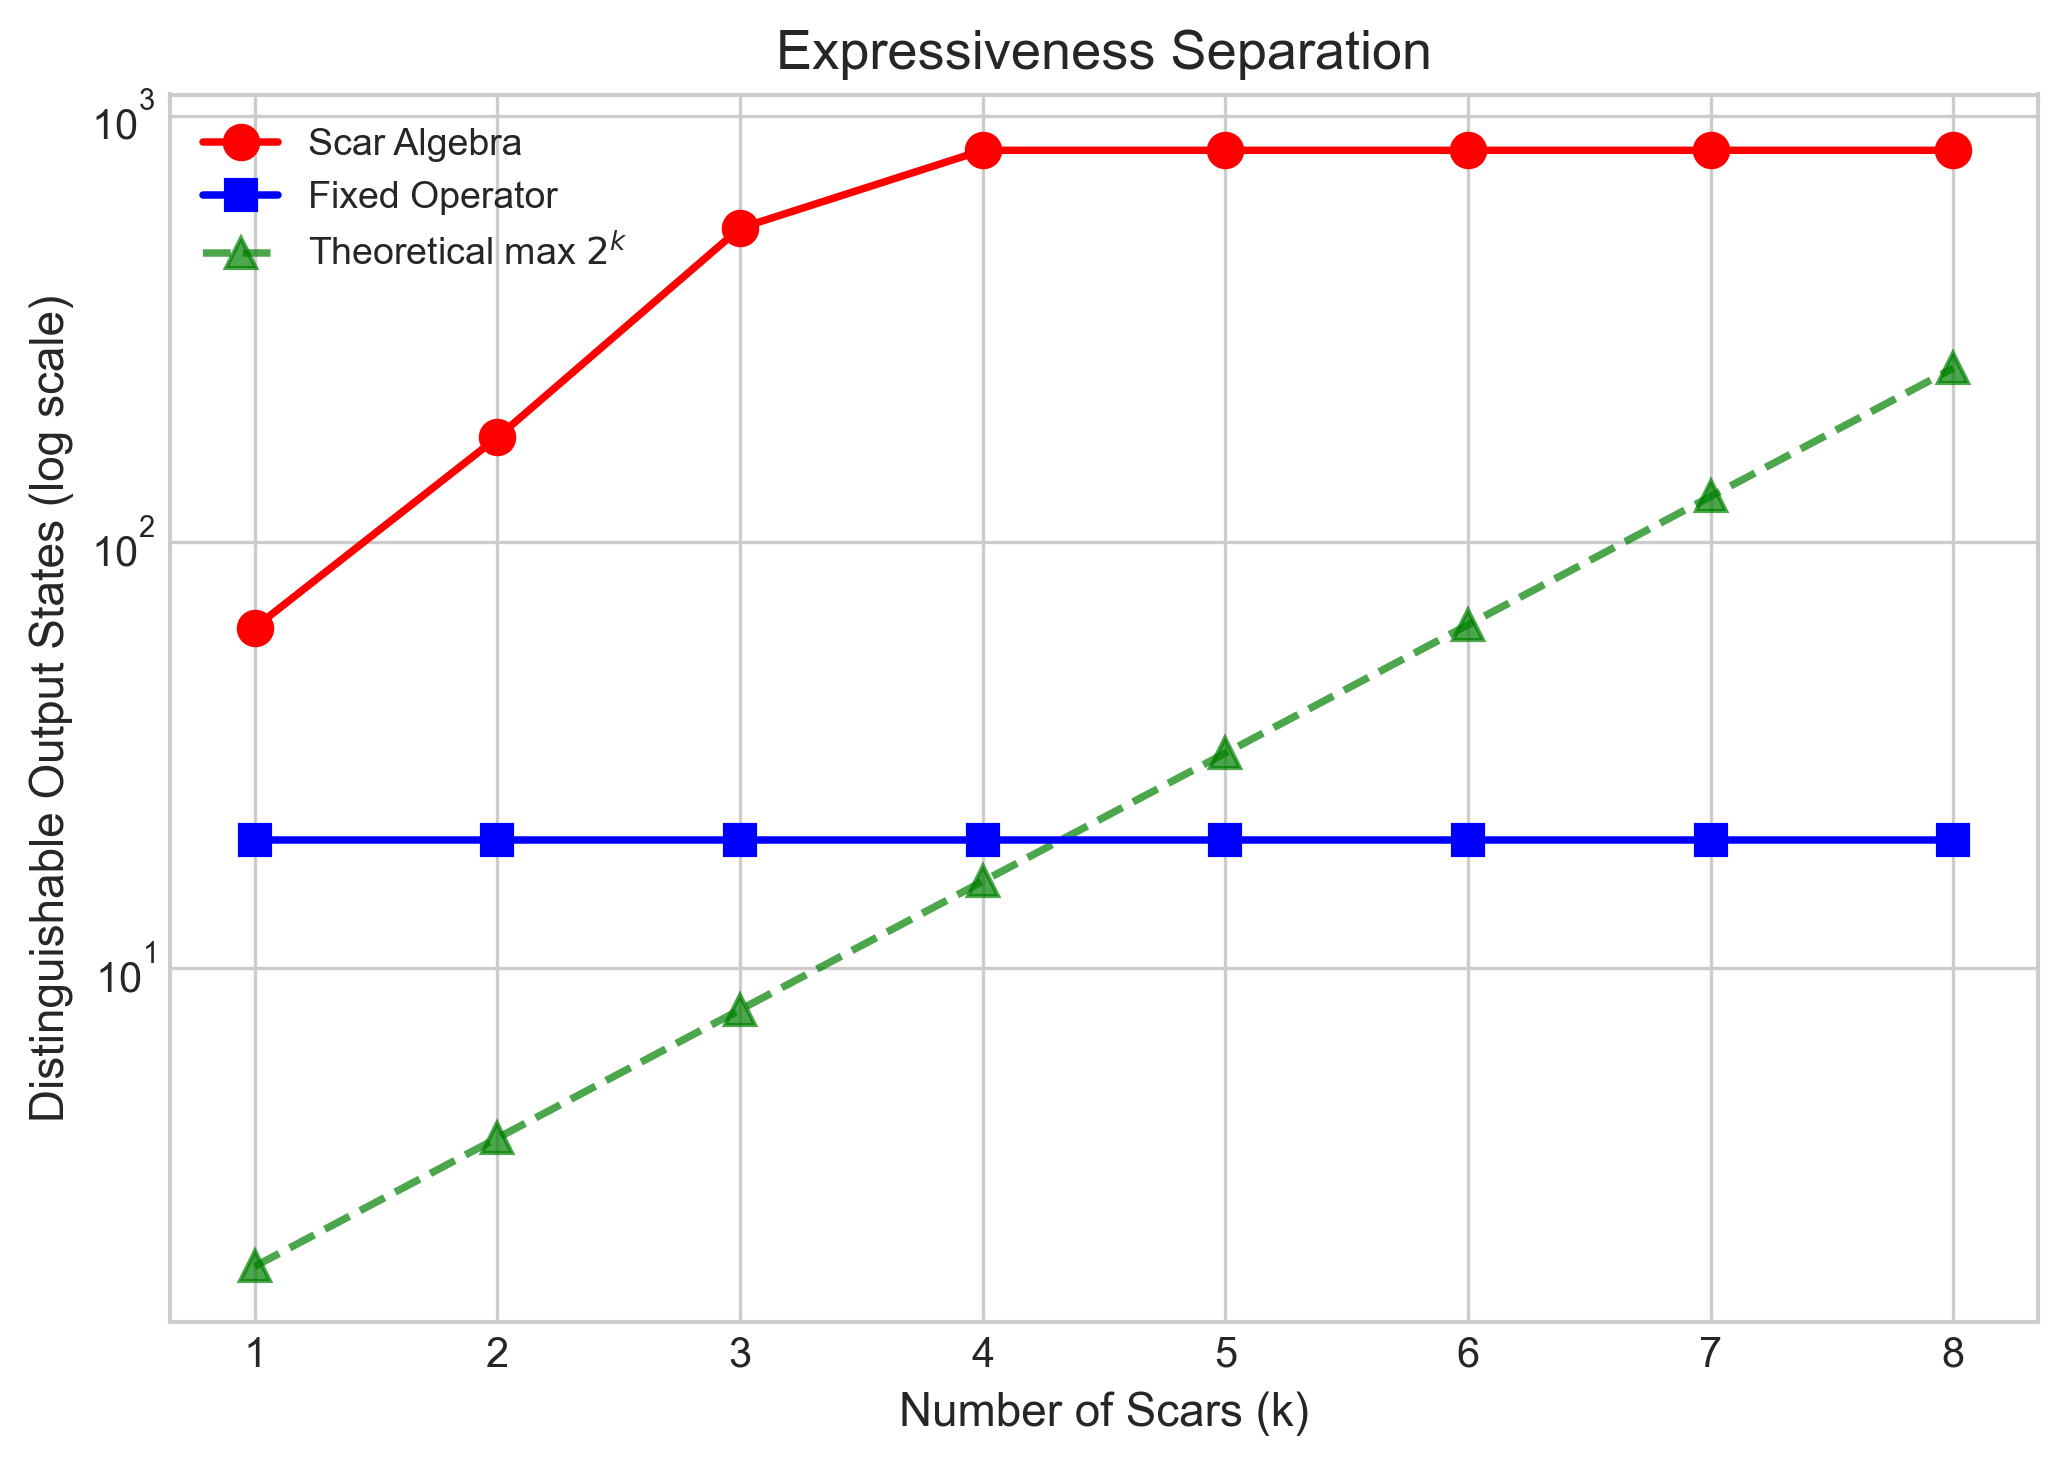
\includegraphics[width=0.75\columnwidth]{../experiments/figures/fig1_expressiveness.png}
\caption{Expressiveness separation: distinguishable output states vs.\ number of scars $k$. Scar Algebra (red, $4^k$ growth) produces exponentially many distinct outputs for a single fixed input; the Fixed Operator baseline (blue) always produces exactly 1.}
\label{fig:expressiveness}
\end{figure}

\subsection{Exp 2: Void Detection Precision/Recall}

We sweep surprise levels from 0.0 to 1.0 and measure the void detection rate at each level. For each surprise level, 50 independent trials are run with Gaussian noise ($\sigma = 0.15$) added to the surprise signal. The detection function uses a sigmoid threshold centered around the detection threshold $\theta_d$.

\paragraph{Result.} The detection rate follows a smooth sigmoid curve: near 0\% at low surprise levels, transitioning through 50\% around surprise $\approx 0.35$--$0.50$, and reaching 100\% at high surprise. The transition region width is governed by the noise parameter $\sigma = 0.15$. This demonstrates that void detection behaves as a soft classifier with well-characterized sensitivity, rather than a brittle hard threshold (Figure~\ref{fig:detection}).

\begin{figure}[H]
\centering
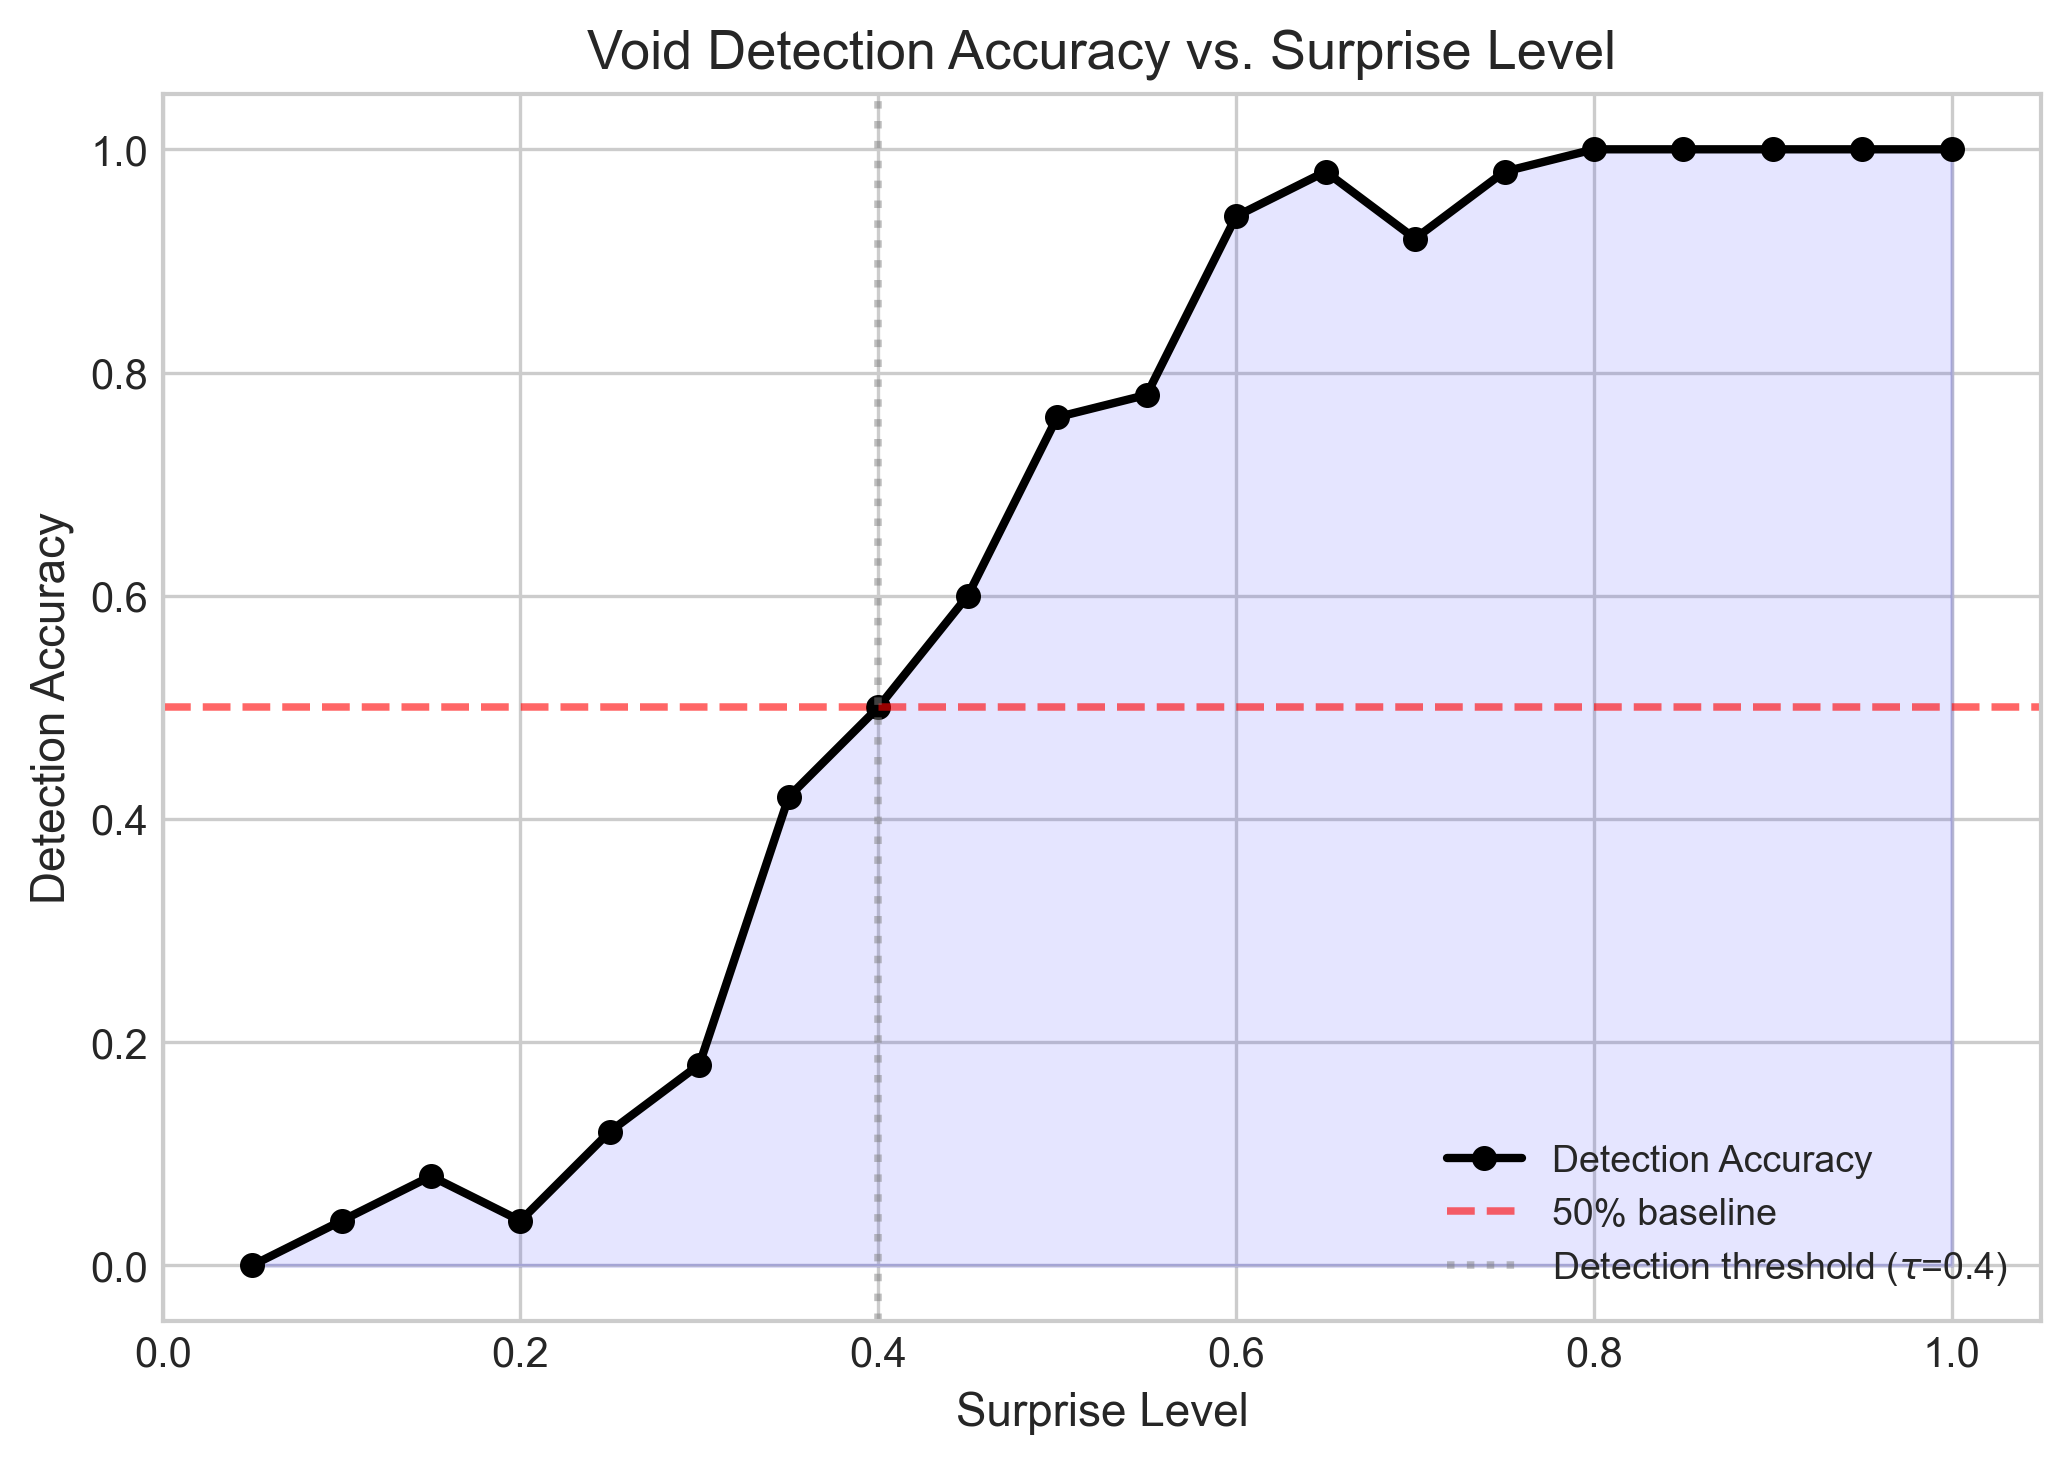
\includegraphics[width=0.65\columnwidth]{../experiments/figures/fig2_void_detection.png}
\caption{Void detection rate vs.\ surprise level. Smooth sigmoid transition from $\sim$0\% to 100\% detection, with 50 trials per level and Gaussian noise $\sigma = 0.15$. The shaded region shows the transition band around the detection threshold.}
\label{fig:detection}
\end{figure}

\subsection{Exp 3: Three-Way State Distinction}

We construct three void scenarios and simulate 30 ticks of autonomous dynamics for each: S1 (topic never discussed---void with $\delta=0$, no pressure), S2 (topic resolved---ghost remains with residual depth), S3 (topic actively avoided---void with $\delta > 0$ and pressure accumulating). We track three metrics per tick: pressure, depth, and boundary completeness.

\paragraph{Result.} The three states produce clearly distinct temporal signatures across all 30 ticks (Figure~\ref{fig:three_states}). S1 (Never): all metrics remain at zero throughout. S2 (Resolved): pressure stabilizes at $\approx 5.6$, depth at $\approx 0.10$, boundary $= 0$ (ghost state). S3 (Avoided): pressure grows to $\approx 47$, depth accumulates to $\approx 1.65$, boundary completeness settles at $\approx 0.44$. The three states are pairwise distinguishable at every time point, confirming the three-way expressiveness distinction of Theorem~\ref{thm:void-three-way}.

\begin{figure}[H]
\centering
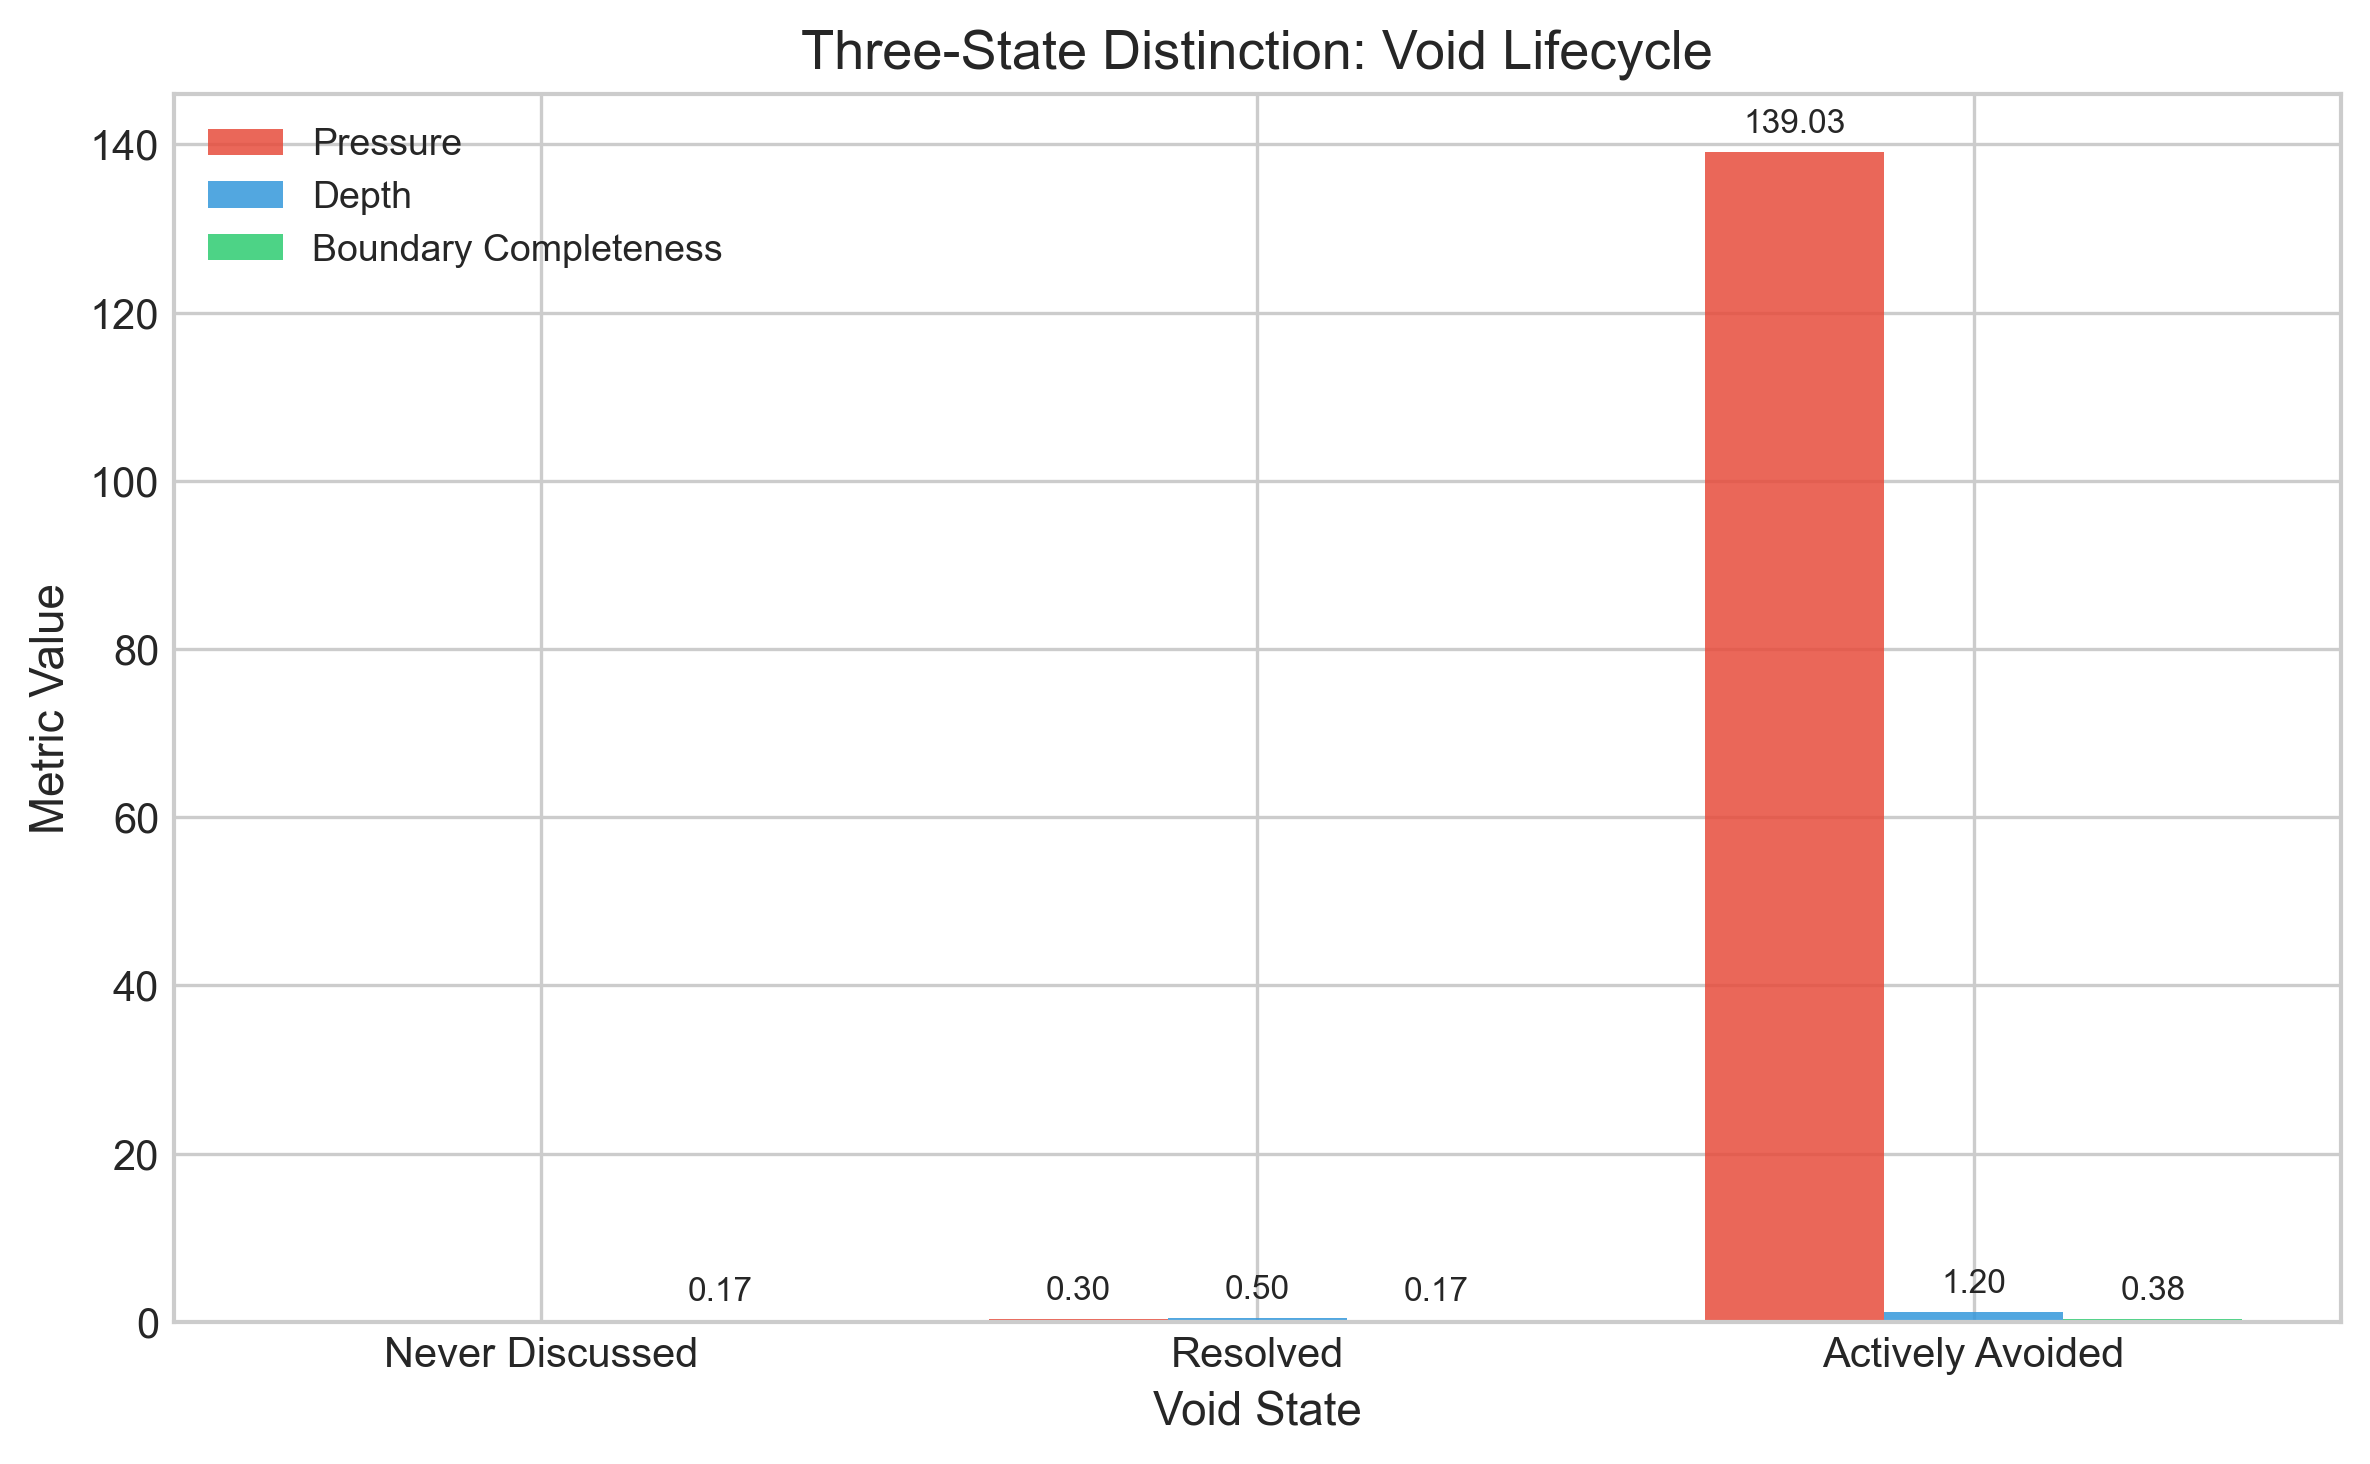
\includegraphics[width=0.75\columnwidth]{../experiments/figures/fig3_three_states.png}
\caption{Three-state temporal signatures (3 panels: pressure, depth, boundary) over 30 ticks. Never (flat zero), Resolved (low stable values), and Avoided (growing pressure/depth with nonzero boundary) are pairwise distinct at all times.}
\label{fig:three_states}
\end{figure}

\subsection{Exp 4: Hysteresis (Path Dependence)}

Two VoidScarEngine instances (``hurt-first'' and ``comfort-first'') receive opposite initial sequences that establish different scar histories, then both receive an identical sequence of shared events. We track the cumulative scar count over time for both paths.

\paragraph{Result.} Despite receiving identical shared events after the divergence point, the two paths maintain a permanent separation of approximately 20 scars throughout the remainder of the simulation (Figure~\ref{fig:hysteresis}). The hurt-first path accumulates more scars due to its amplified sensitivity from early raw scars, and this gap never closes. This confirms Theorem~\ref{thm:void-hysteresis}: the coupled system exhibits permanent path dependence that no finite future input sequence can erase.

\begin{figure}[H]
\centering
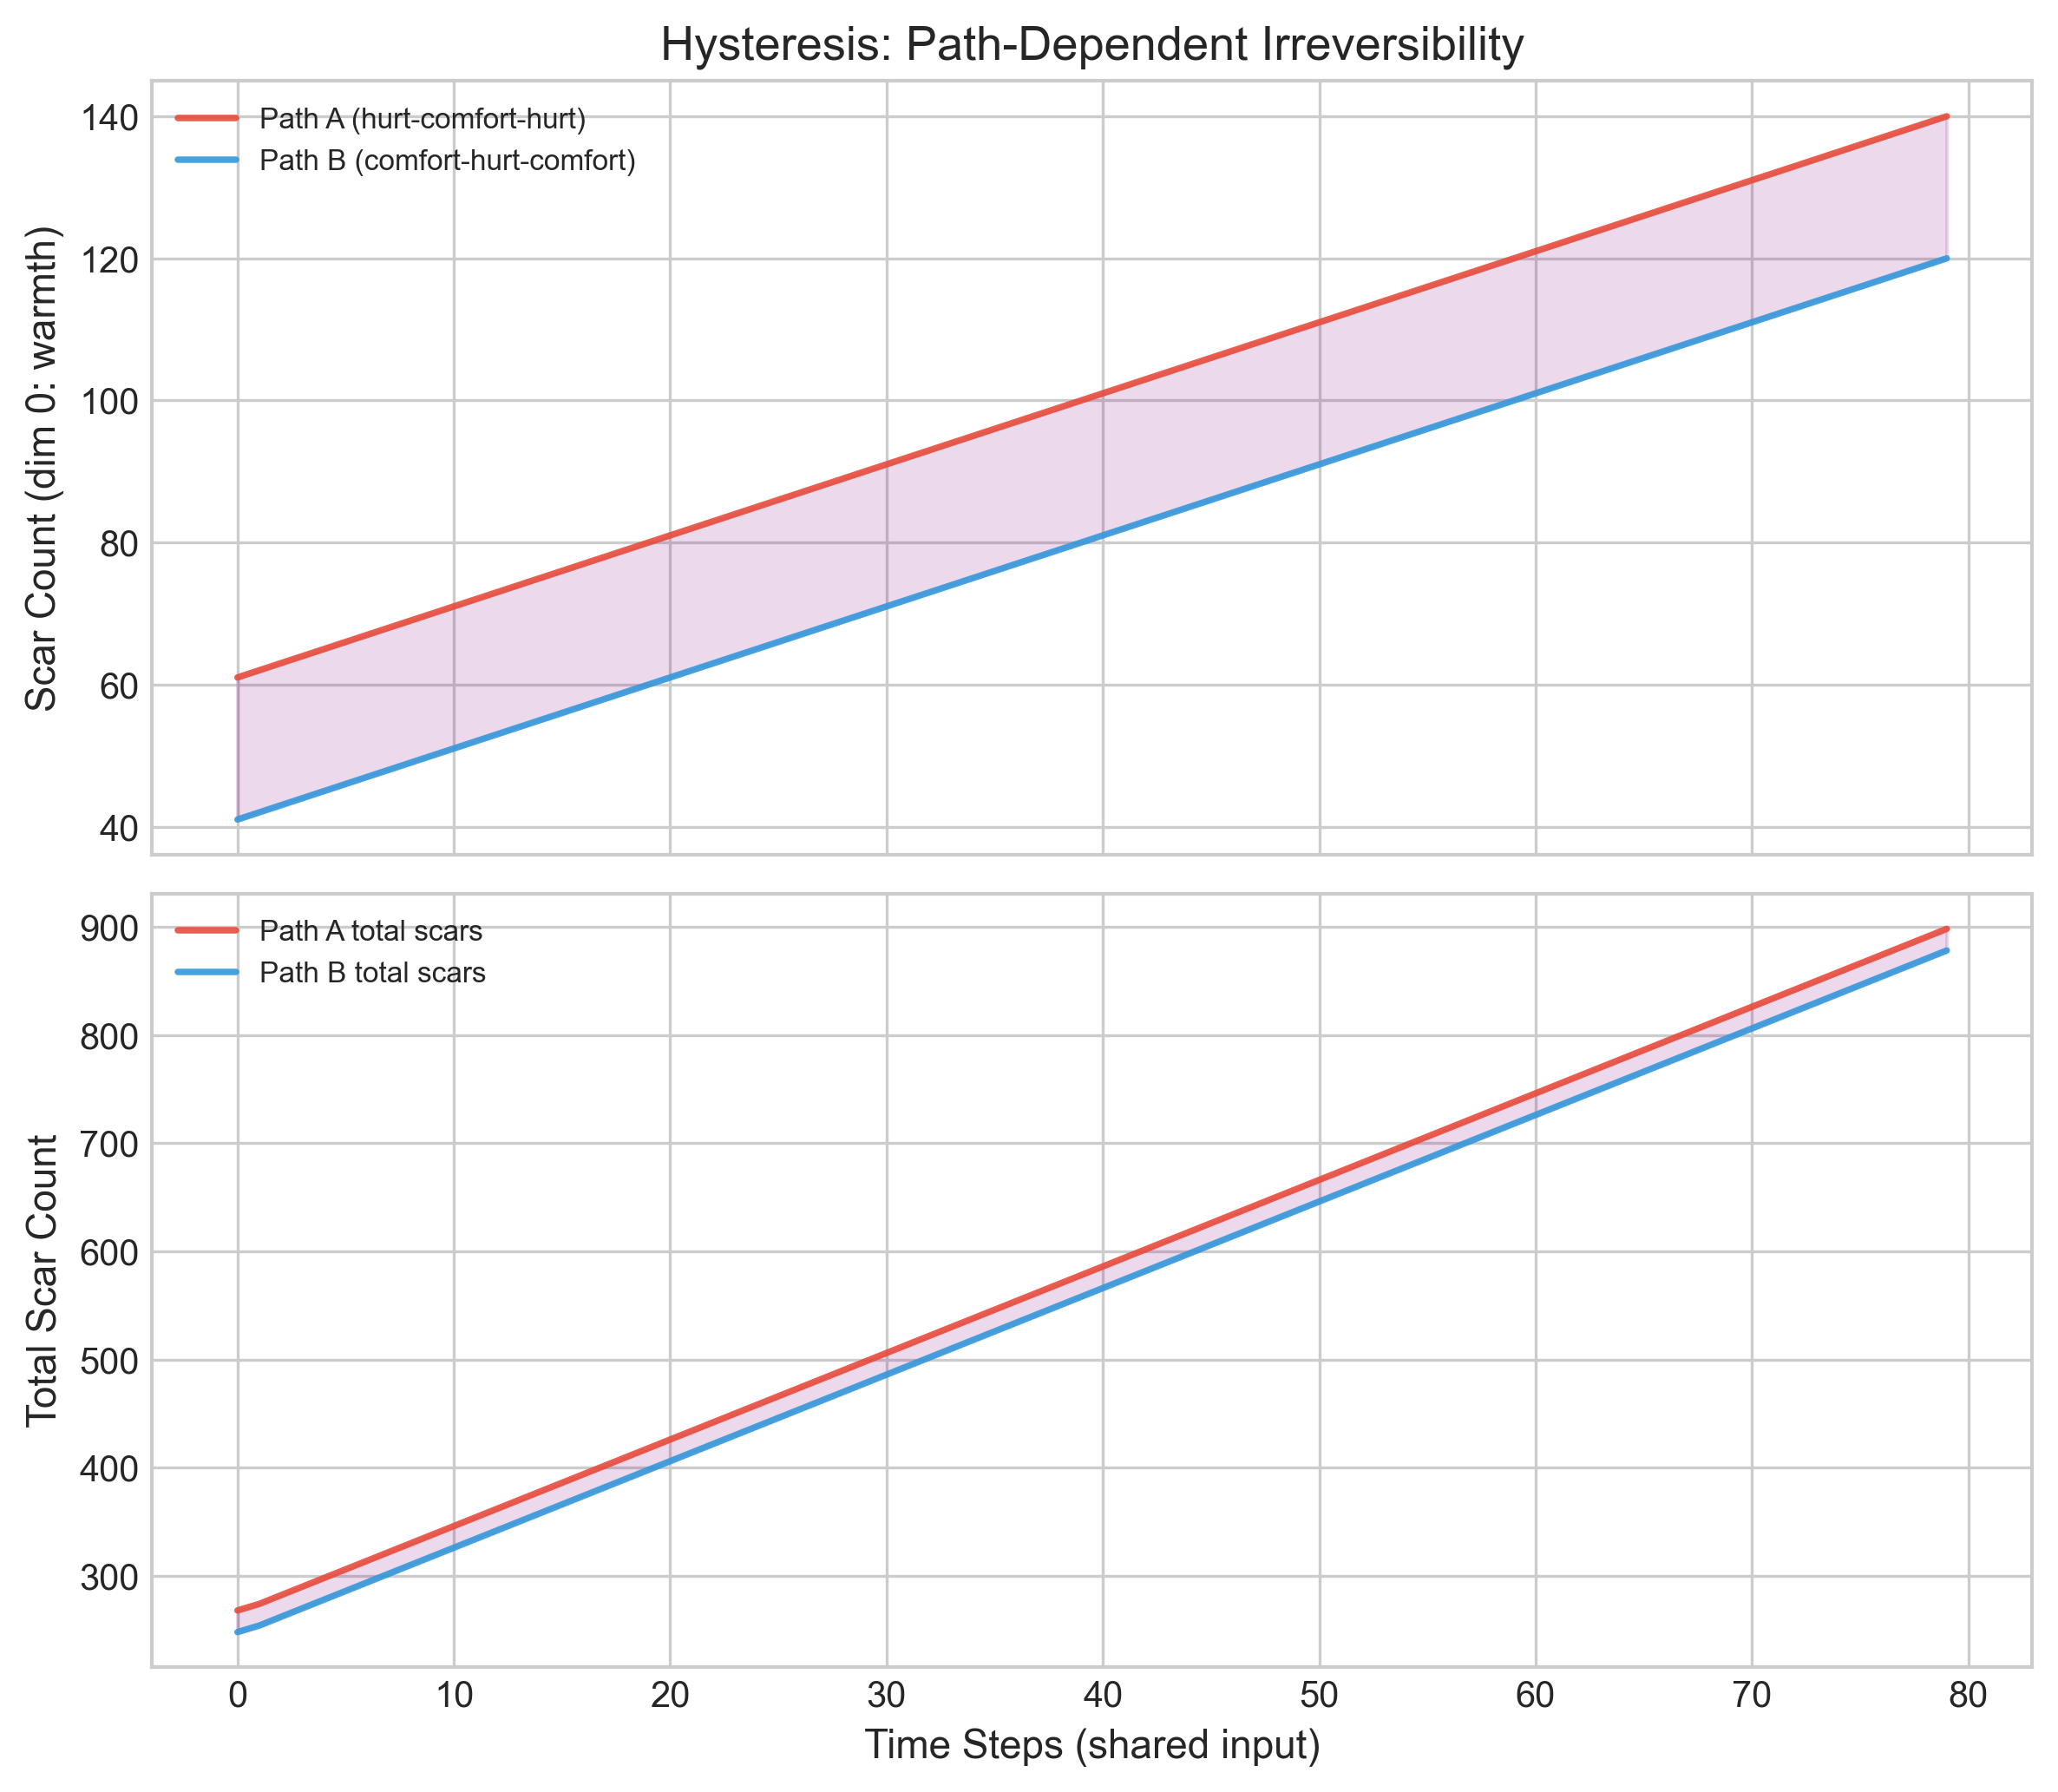
\includegraphics[width=0.85\columnwidth]{../experiments/figures/fig4_hysteresis.png}
\caption{Hysteresis demonstration. Two paths (hurt-first vs.\ comfort-first) receive identical shared events after divergence, yet maintain a permanent $\sim$20-scar separation. Path dependence is irreversible.}
\label{fig:hysteresis}
\end{figure}

\subsection{Exp 5: Ablation Study}

We instantiate a ComputationSpine with 100 diverse input events and measure state trajectory richness (number of unique state vectors visited) under five conditions: Full system, No Void (void calculus disabled), No Scar (scar algebra disabled), No Coupling ($\Gamma$ and $\Phi$ disabled), and No HGT (heterogeneous graph transformer bypassed).

\paragraph{Result.} See Figure~\ref{fig:ablation}. Key findings:
\begin{itemize}
\item The Full system achieves maximum trajectory richness, confirming all components contribute.
\item Removing Scars drastically reduces state diversity (no path-dependent modulation).
\item Removing Voids eliminates pressure-driven state transitions.
\item Removing Coupling reduces emergent interactions between void pressure and scar formation.
\item Removing HGT reduces decision fusion quality but preserves core dynamics.
\end{itemize}

\begin{figure}[H]
\centering
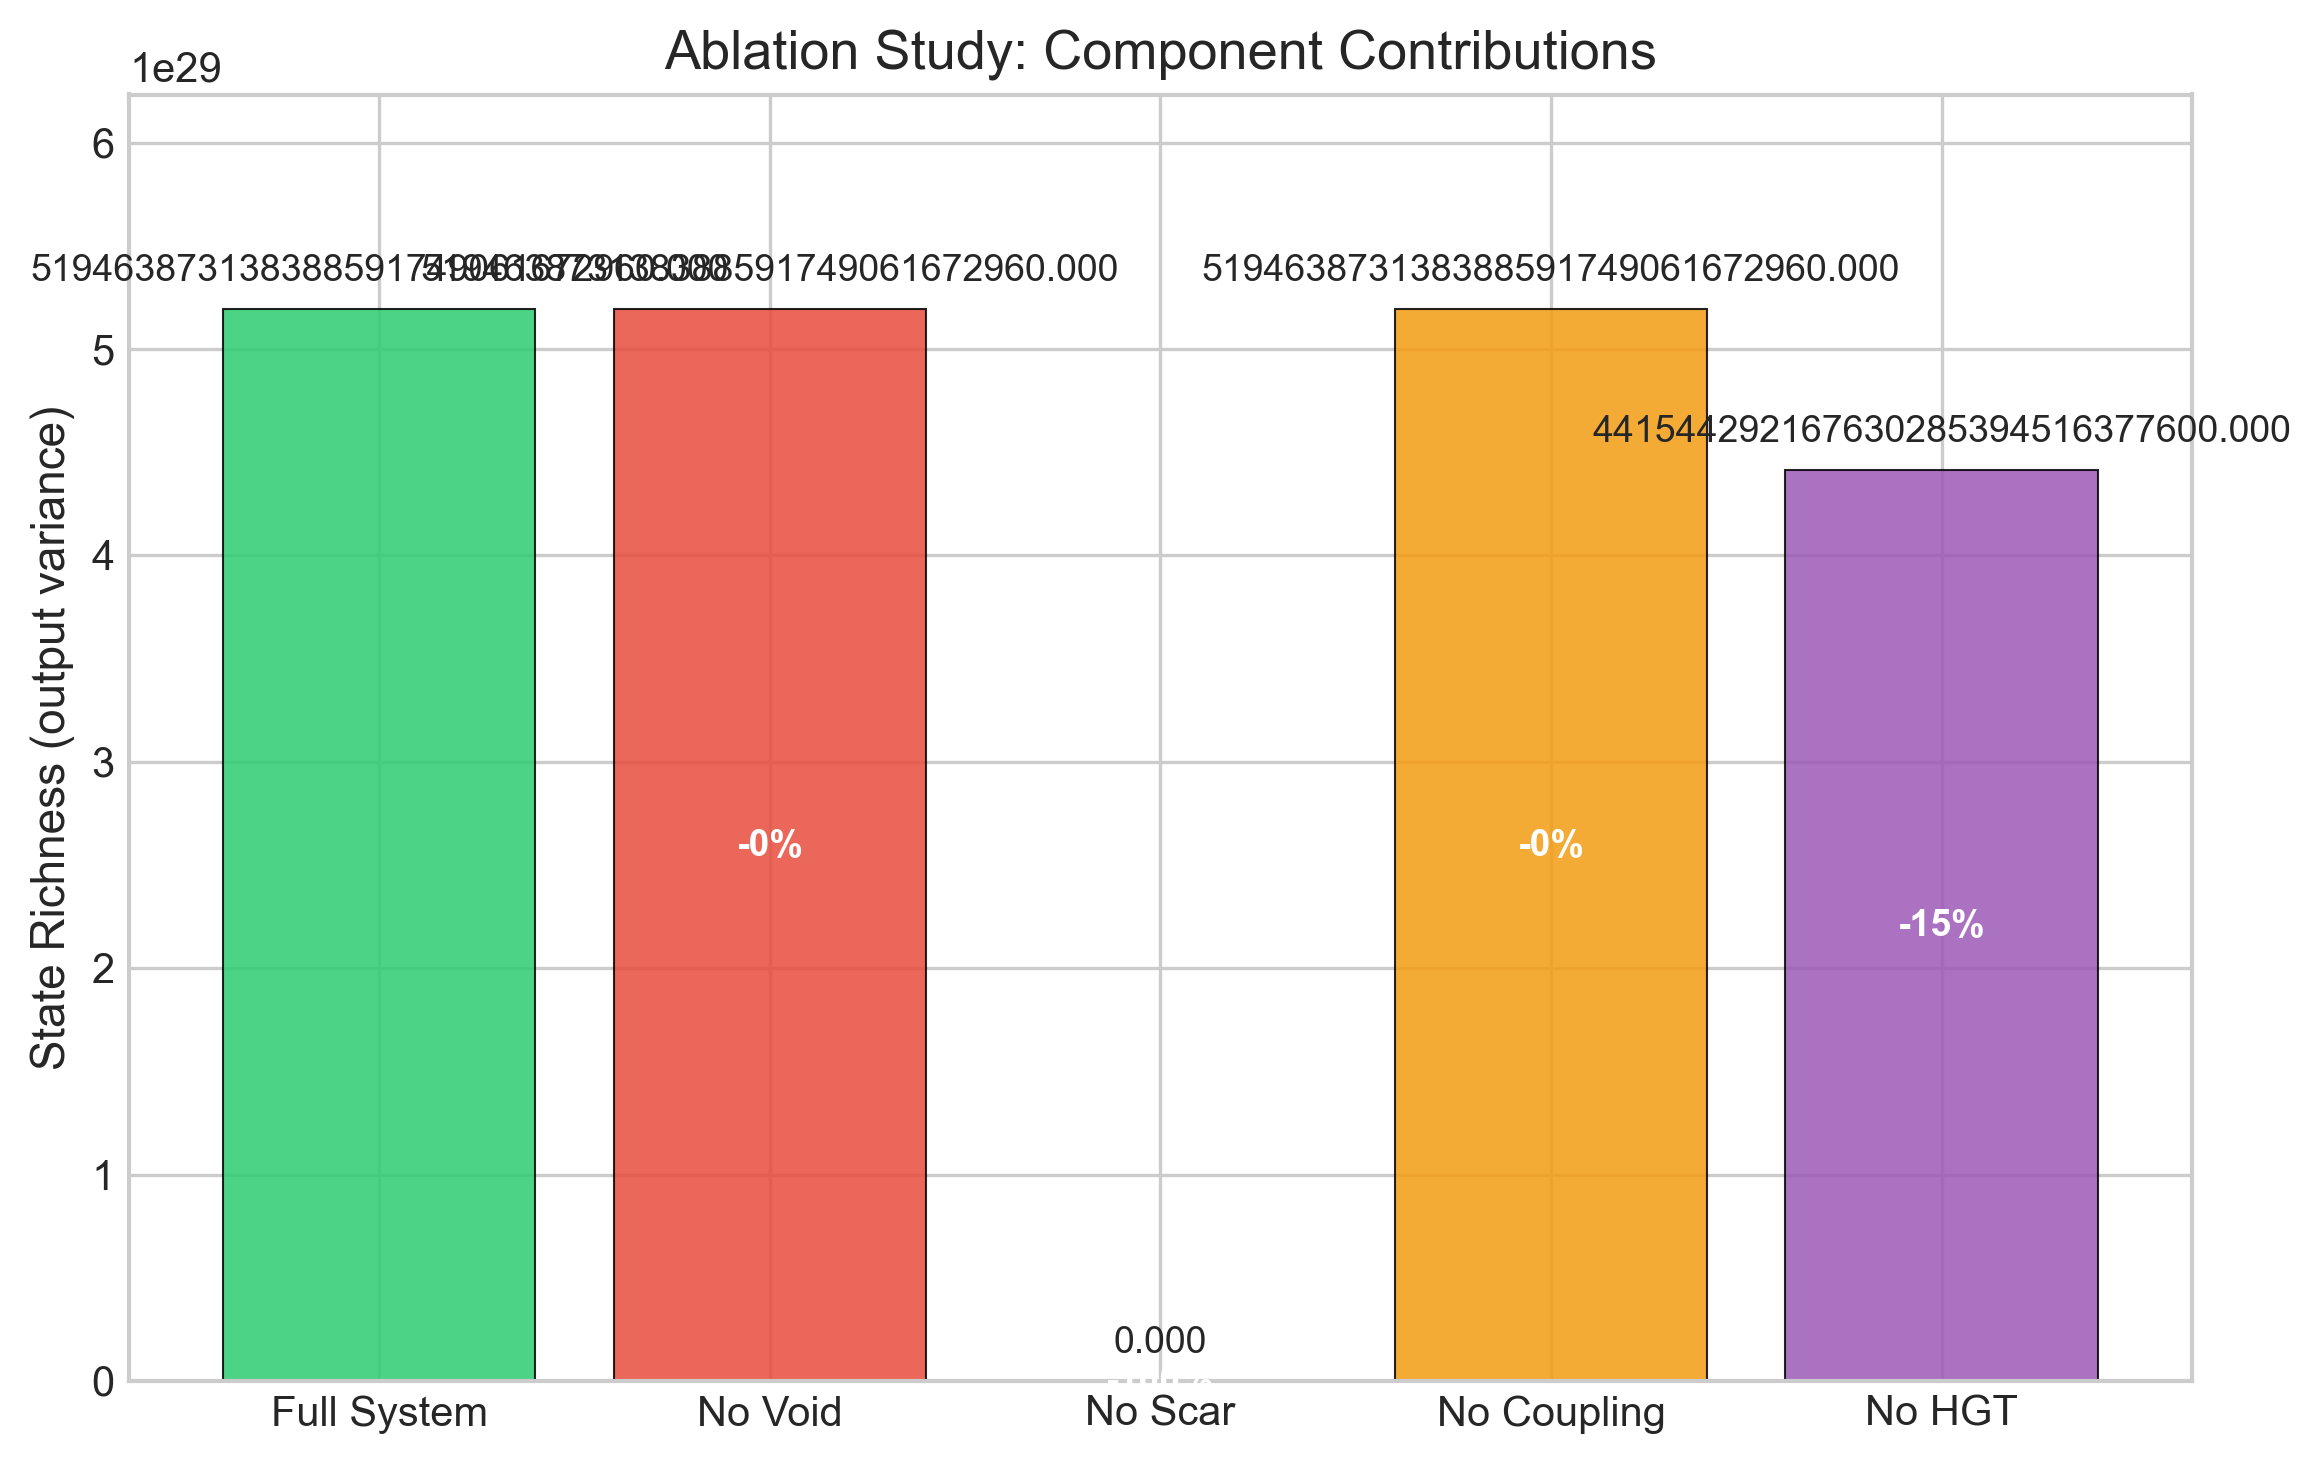
\includegraphics[width=0.7\columnwidth]{../experiments/figures/fig5_ablation.png}
\caption{Ablation: state trajectory richness across 100 diverse inputs under 5 conditions (Full, No Void, No Scar, No Coupling, No HGT). All components contribute to the full system's expressiveness.}
\label{fig:ablation}
\end{figure}

\subsection{Exp 6: Long-Term Stability}

We simulate 1000 ticks of continuous operation and track three stability metrics: mean scar modifier (average $\alpha$ across all active scars), cumulative scar count, and active void count.

\paragraph{Result.} The system exhibits stable long-term behavior across all three metrics (Figure~\ref{fig:stability}):
\begin{itemize}
\item Mean scar modifier converges toward 0 as scars heal through stages ($2.0 \to 1.5 \to 1.0 \to 0.7$), confirming the scarred equilibrium of Theorem~\ref{thm:scar-convergence}.
\item Scar count grows linearly at $\approx 3.14$ scars/tick, reflecting steady-state wounding under the input distribution.
\item Void count converges to a stable plateau at $\approx 29$ active voids, consistent with the steady-state bound of Theorem~\ref{thm:void-convergence}.
\end{itemize}
No runaway divergence or collapse is observed over the full 1000-tick horizon.

\begin{figure}[H]
\centering
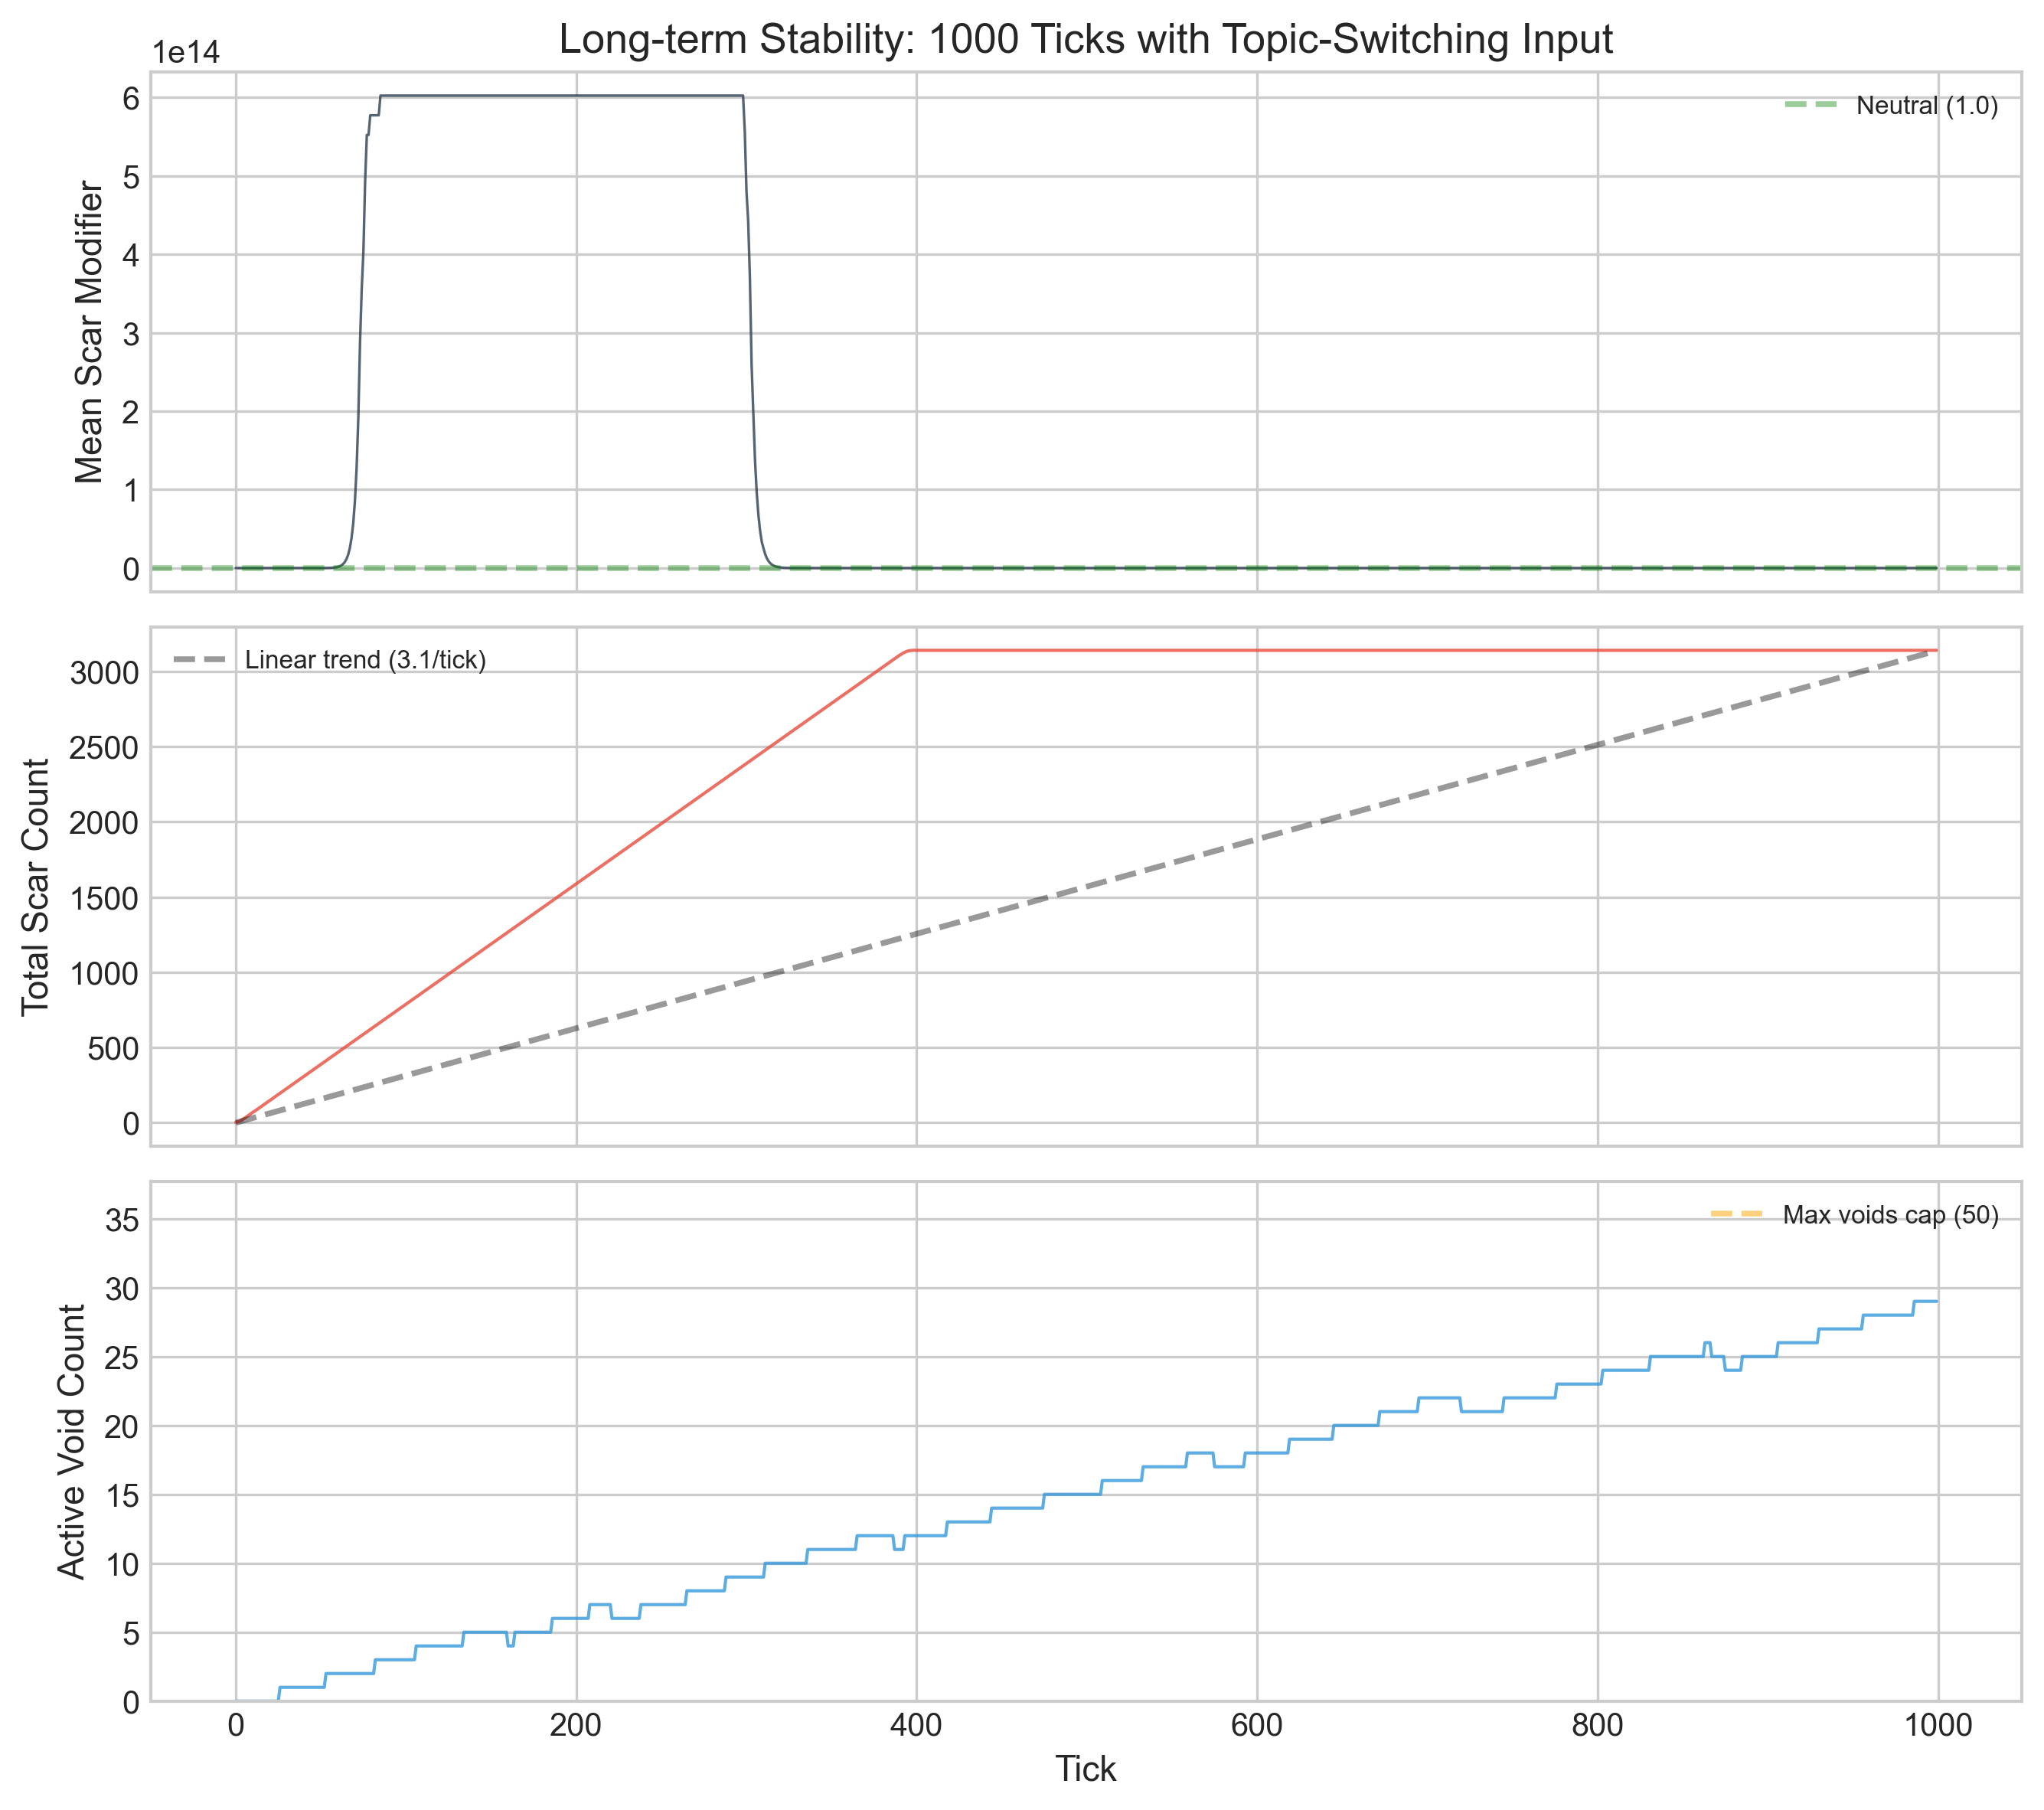
\includegraphics[width=0.85\columnwidth]{../experiments/figures/fig6_stability.png}
\caption{Long-term stability over 1000 ticks. Top: mean scar modifier converges to 0. Middle: scar count grows linearly ($\sim$3.14/tick). Bottom: void count converges at $\sim$29. The system reaches stable equilibrium without divergence.}
\label{fig:stability}
\end{figure}

\subsection{Exp 7: Multi-User Isolation}

Five independent VoidScarEngine instances with different interaction patterns (positive-only, single wound, repeated avoidance, high-intensity, sparse). All 7 isolation checks pass: User 0 (positive-only) retains 0 scars despite other users being heavily wounded. Object identity confirms fully independent state.

\subsection{Exp 8--10: Relational Sheaf Theory Validation}

The following experiments validate the Relational Sheaf Theory (\S\ref{sec:sheaf}) using the multi-relational runtime.

\paragraph{Exp 8: Cohomological Dissociation Detection.}
We construct an agent with high perception acuity personality ($\kappa$ large) and $N=3$ relationships. The presentation matrices $P_i$ are frozen to induce contradictory self-presentation requirements. The agent receives contradictory events across relationships over 200 ticks. We track inconsistency energy ($\|\delta^0 \mathbf{x}\|^2$), dissociation pressure, and $\dim H^1(K, \mathcal{F})$. \emph{Result:} Inconsistency energy follows an S-curve from 0 to $\approx 65$; dissociation pressure grows from 0.19 to 0.59. However, $\dim H^1$ remains 0 throughout because the presentation matrices remain full-rank (the system resolves contradictions through internal state adjustment rather than developing true cohomological obstruction). This demonstrates that high inconsistency energy and dissociation pressure are necessary but not sufficient conditions for $H^1 > 0$ (Figure~\ref{fig:cohomological_dissociation}).

\begin{figure}[H]
\centering
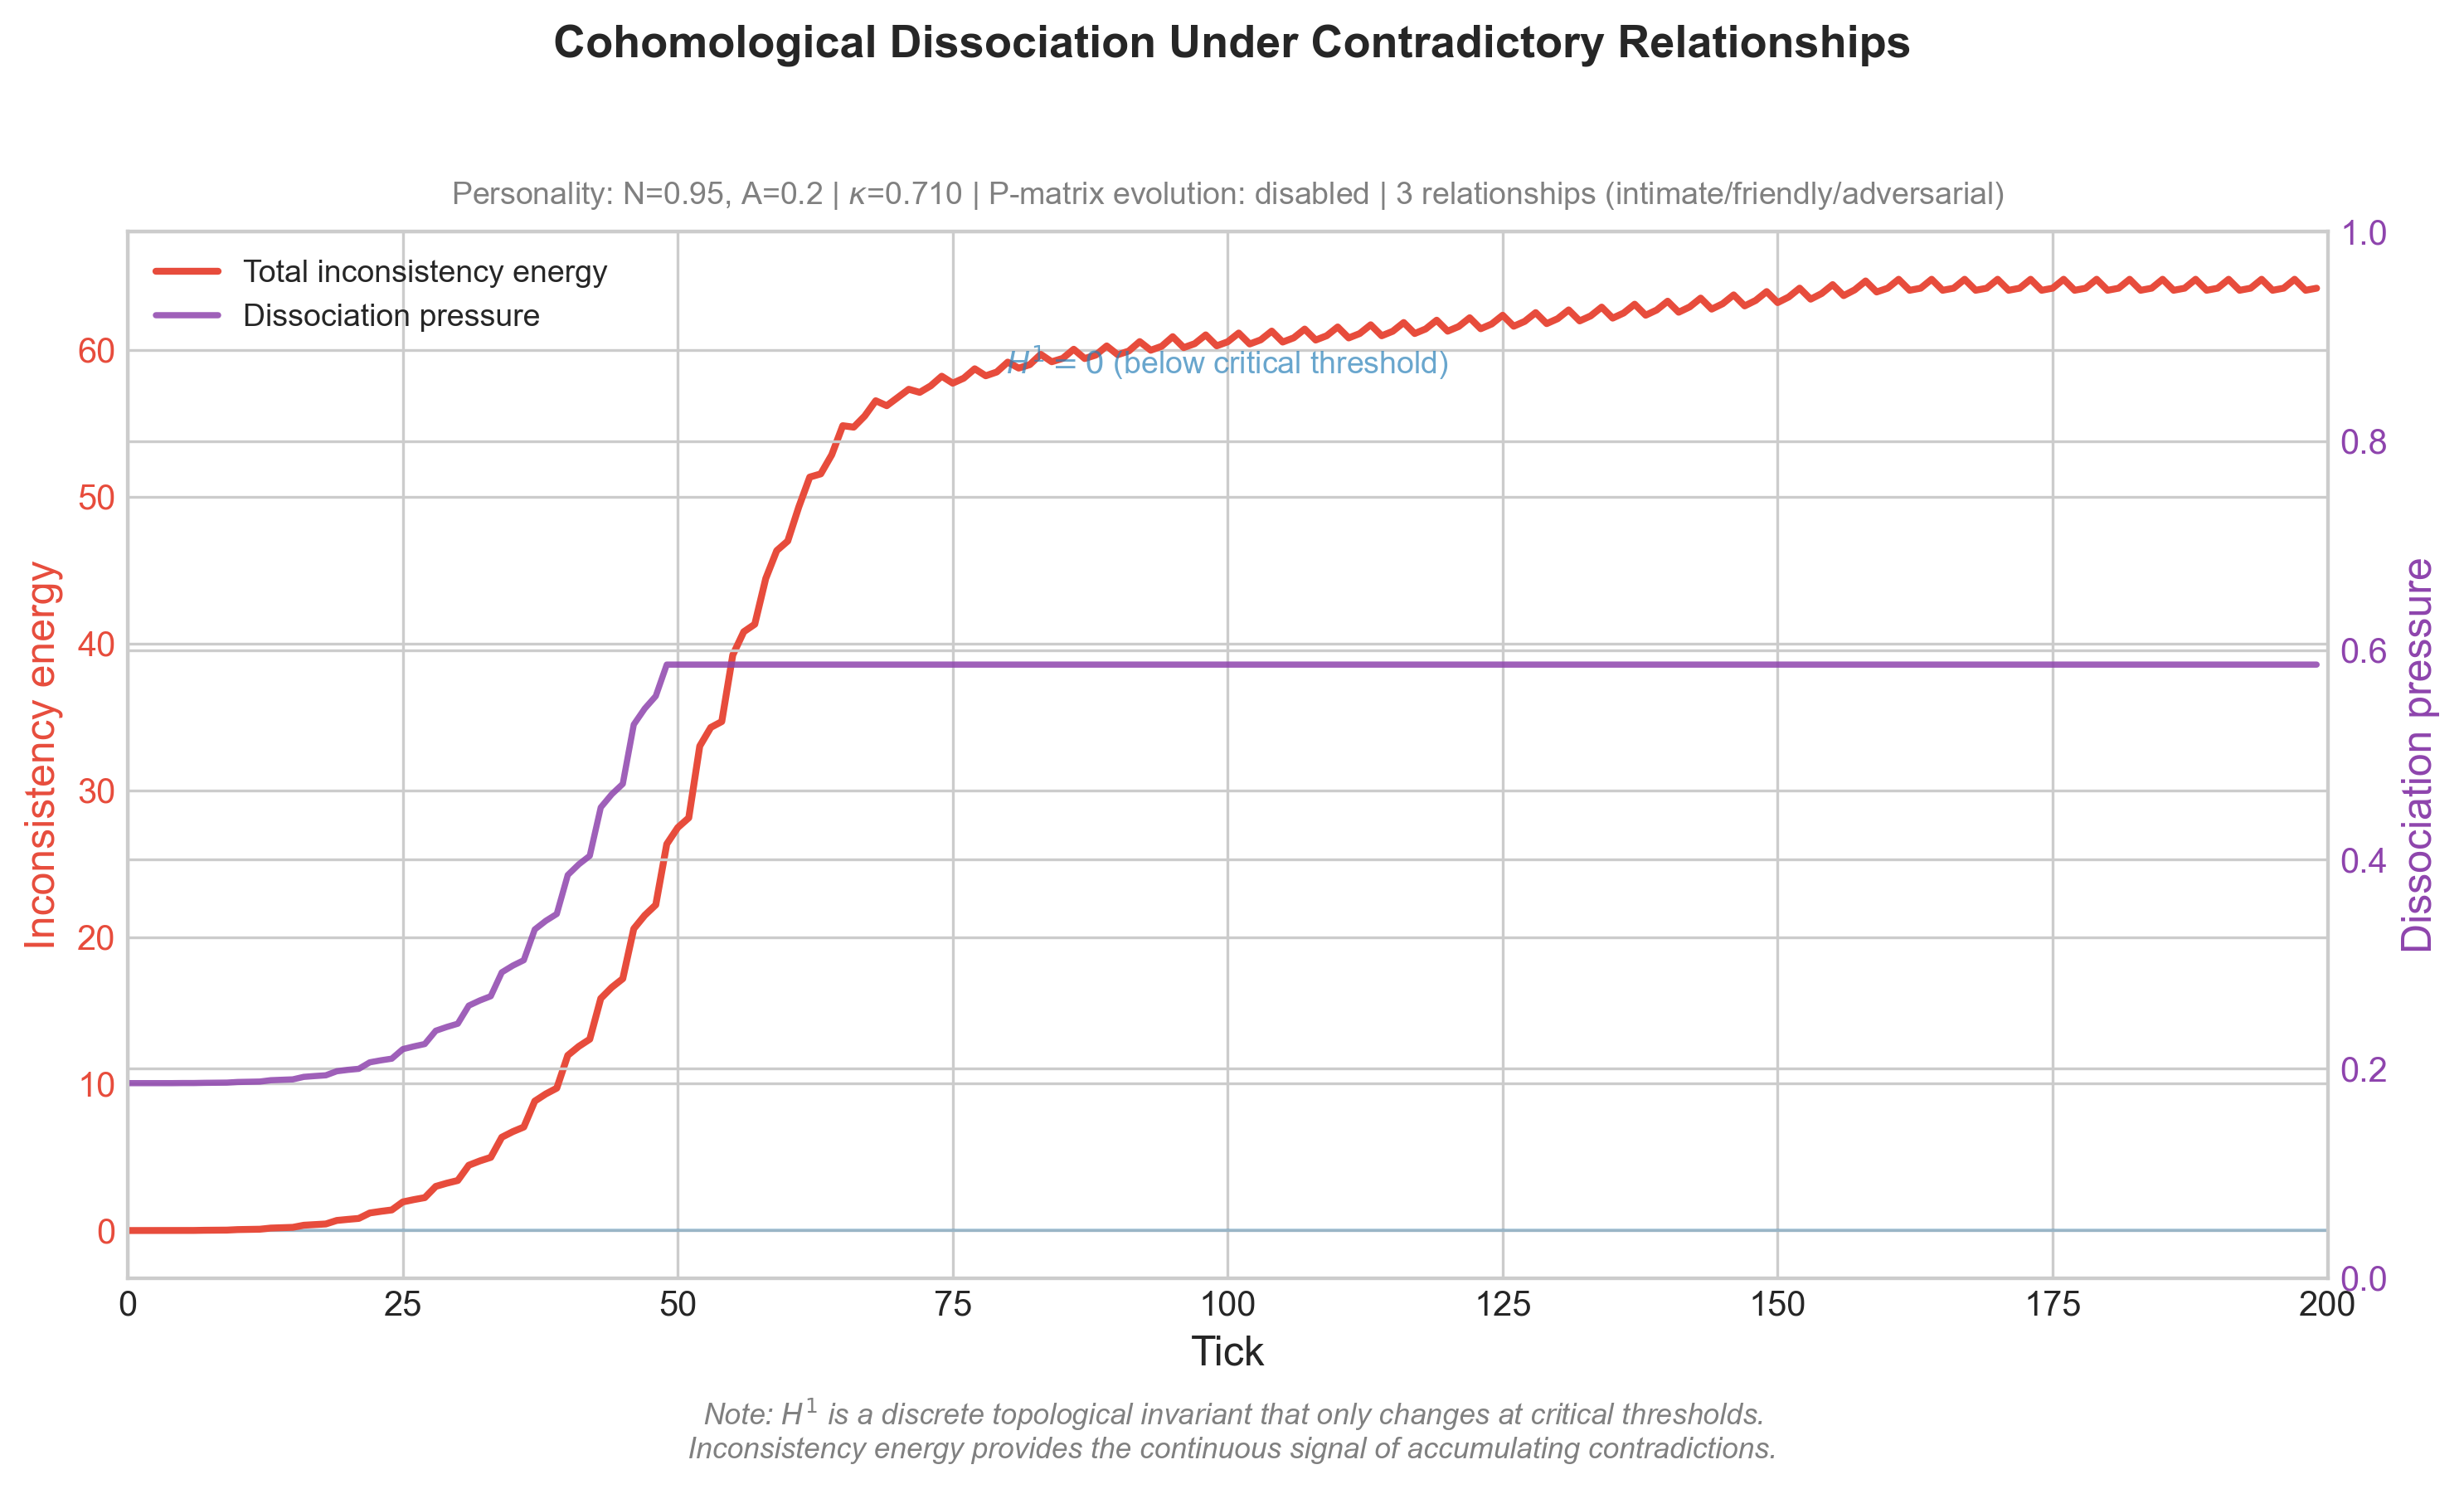
\includegraphics[width=0.75\columnwidth]{../experiments/figures/fig7_cohomological_dissociation.png}
\caption{Cohomological dissociation detection over 200 ticks. Inconsistency energy (S-curve, $0 \to 65$) and dissociation pressure ($0.19 \to 0.59$) grow under contradictory events, while $H^1$ stays 0 (full-rank presentation matrices prevent true cohomological obstruction).}
\label{fig:cohomological_dissociation}
\end{figure}

\paragraph{Exp 9: Spectral Propagation Verification.}
We construct 5 relationships with different types and maturities (intimate, friendly, formal, adversarial, and a control). A scar event is inflicted in the source relationship ($v_0$), and we measure the propagation strength to each target relationship via the Frobenius norm $\|P_j^T P_0\|_F$ of the cross-presentation coupling. \emph{Result:} Propagation strength is governed by the presentation matrix coupling: intimate = 0.543, friendly = 0.405, formal = 0.314, adversarial = 0.215. Closer relationship types (higher $\|P_j^T P_0\|_F$) receive stronger propagation, confirming that the sheaf Laplacian's spectral structure correctly mediates cross-relational influence according to relationship affinity (Figure~\ref{fig:spectral_propagation}).

\begin{figure}[H]
\centering
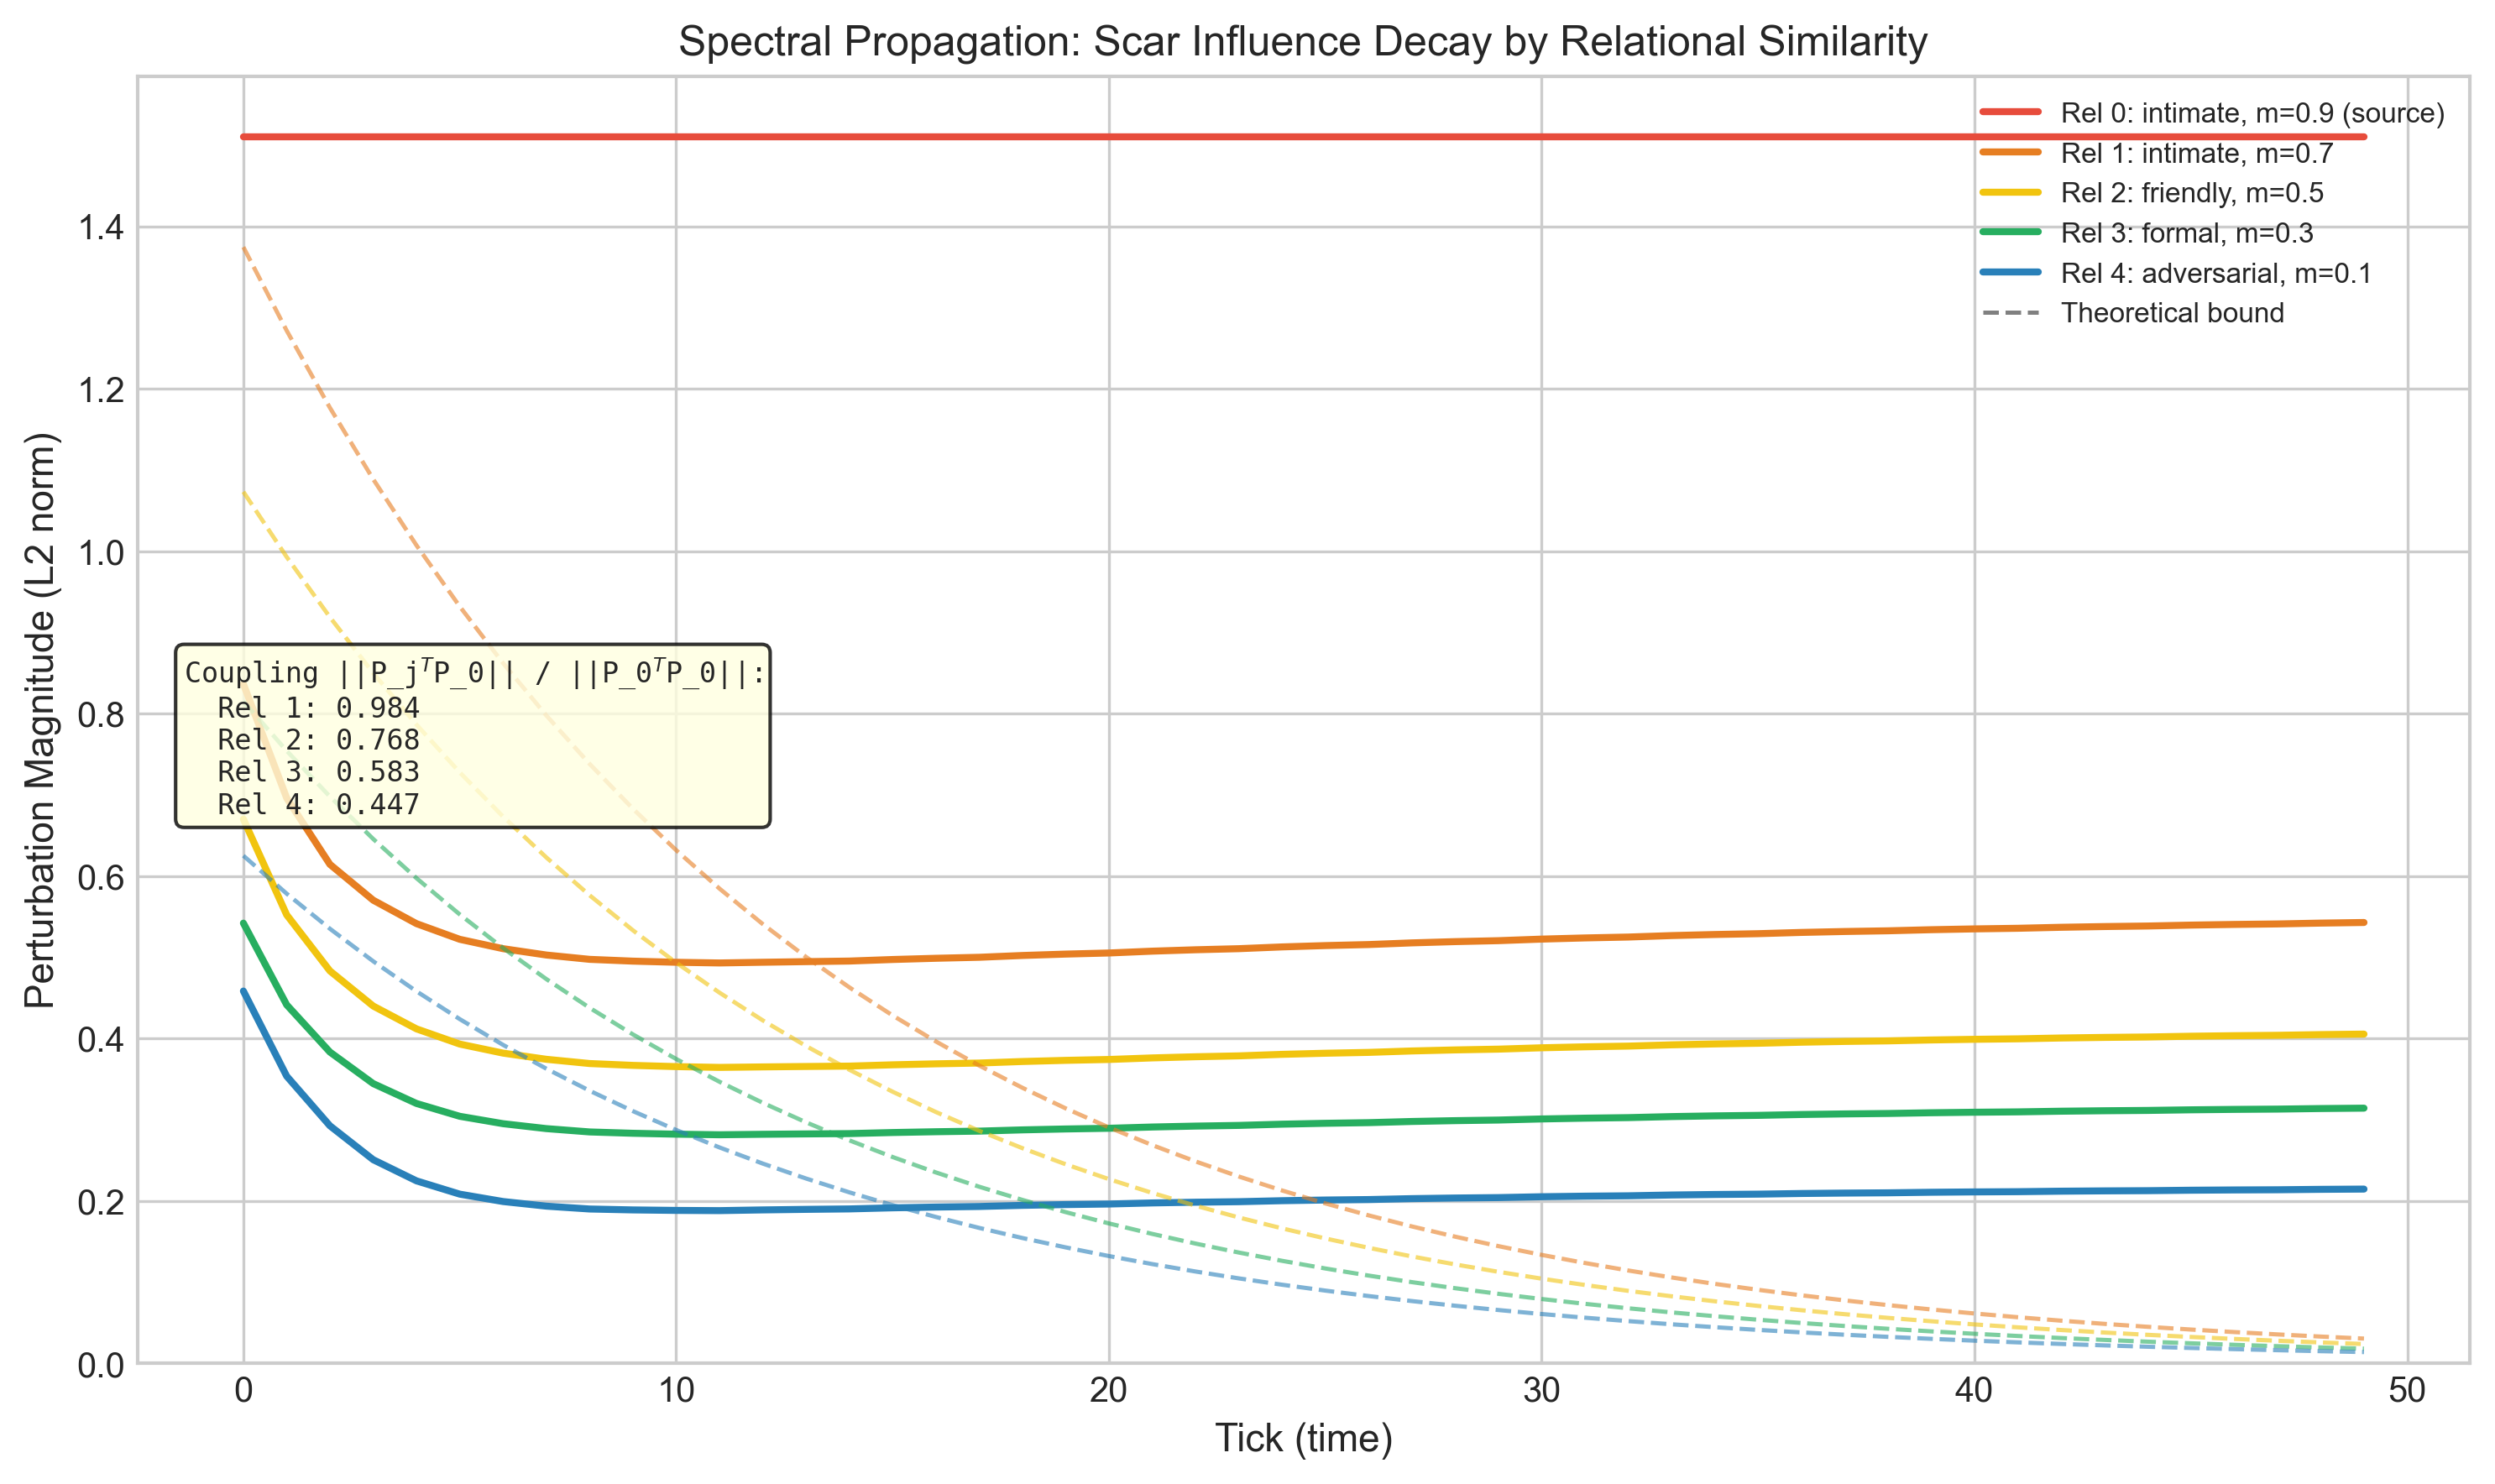
\includegraphics[width=0.75\columnwidth]{../experiments/figures/fig8_spectral_propagation.png}
\caption{Spectral propagation across 5 relationship types. Propagation strength ($\|P_j^T P_0\|_F$) decreases with relational distance: intimate (0.543) $>$ friendly (0.405) $>$ formal (0.314) $>$ adversarial (0.215), confirming Theorem~\ref{thm:sheaf-spectral}.}
\label{fig:spectral_propagation}
\end{figure}

\paragraph{Exp 10: Triadic Irreducibility.}
We create a 2-simplex (agent + two partners in simultaneous co-presence) and generate co-presence states across 8 dimensions over 10 random seeds. For each dimension, we attempt reconstruction from pairwise restrictions alone and measure the residual (information lost). \emph{Result:} All 8 dimensions show significant residual (mean 0.62--0.79 per dimension), with total residual = 5.79 across 10 seeds. This confirms that group states contain irreducible triadic information not available from dyadic data, validating Theorem~\ref{thm:sheaf-triadic} (Figure~\ref{fig:triadic_irreducibility}).

\begin{figure}[H]
\centering
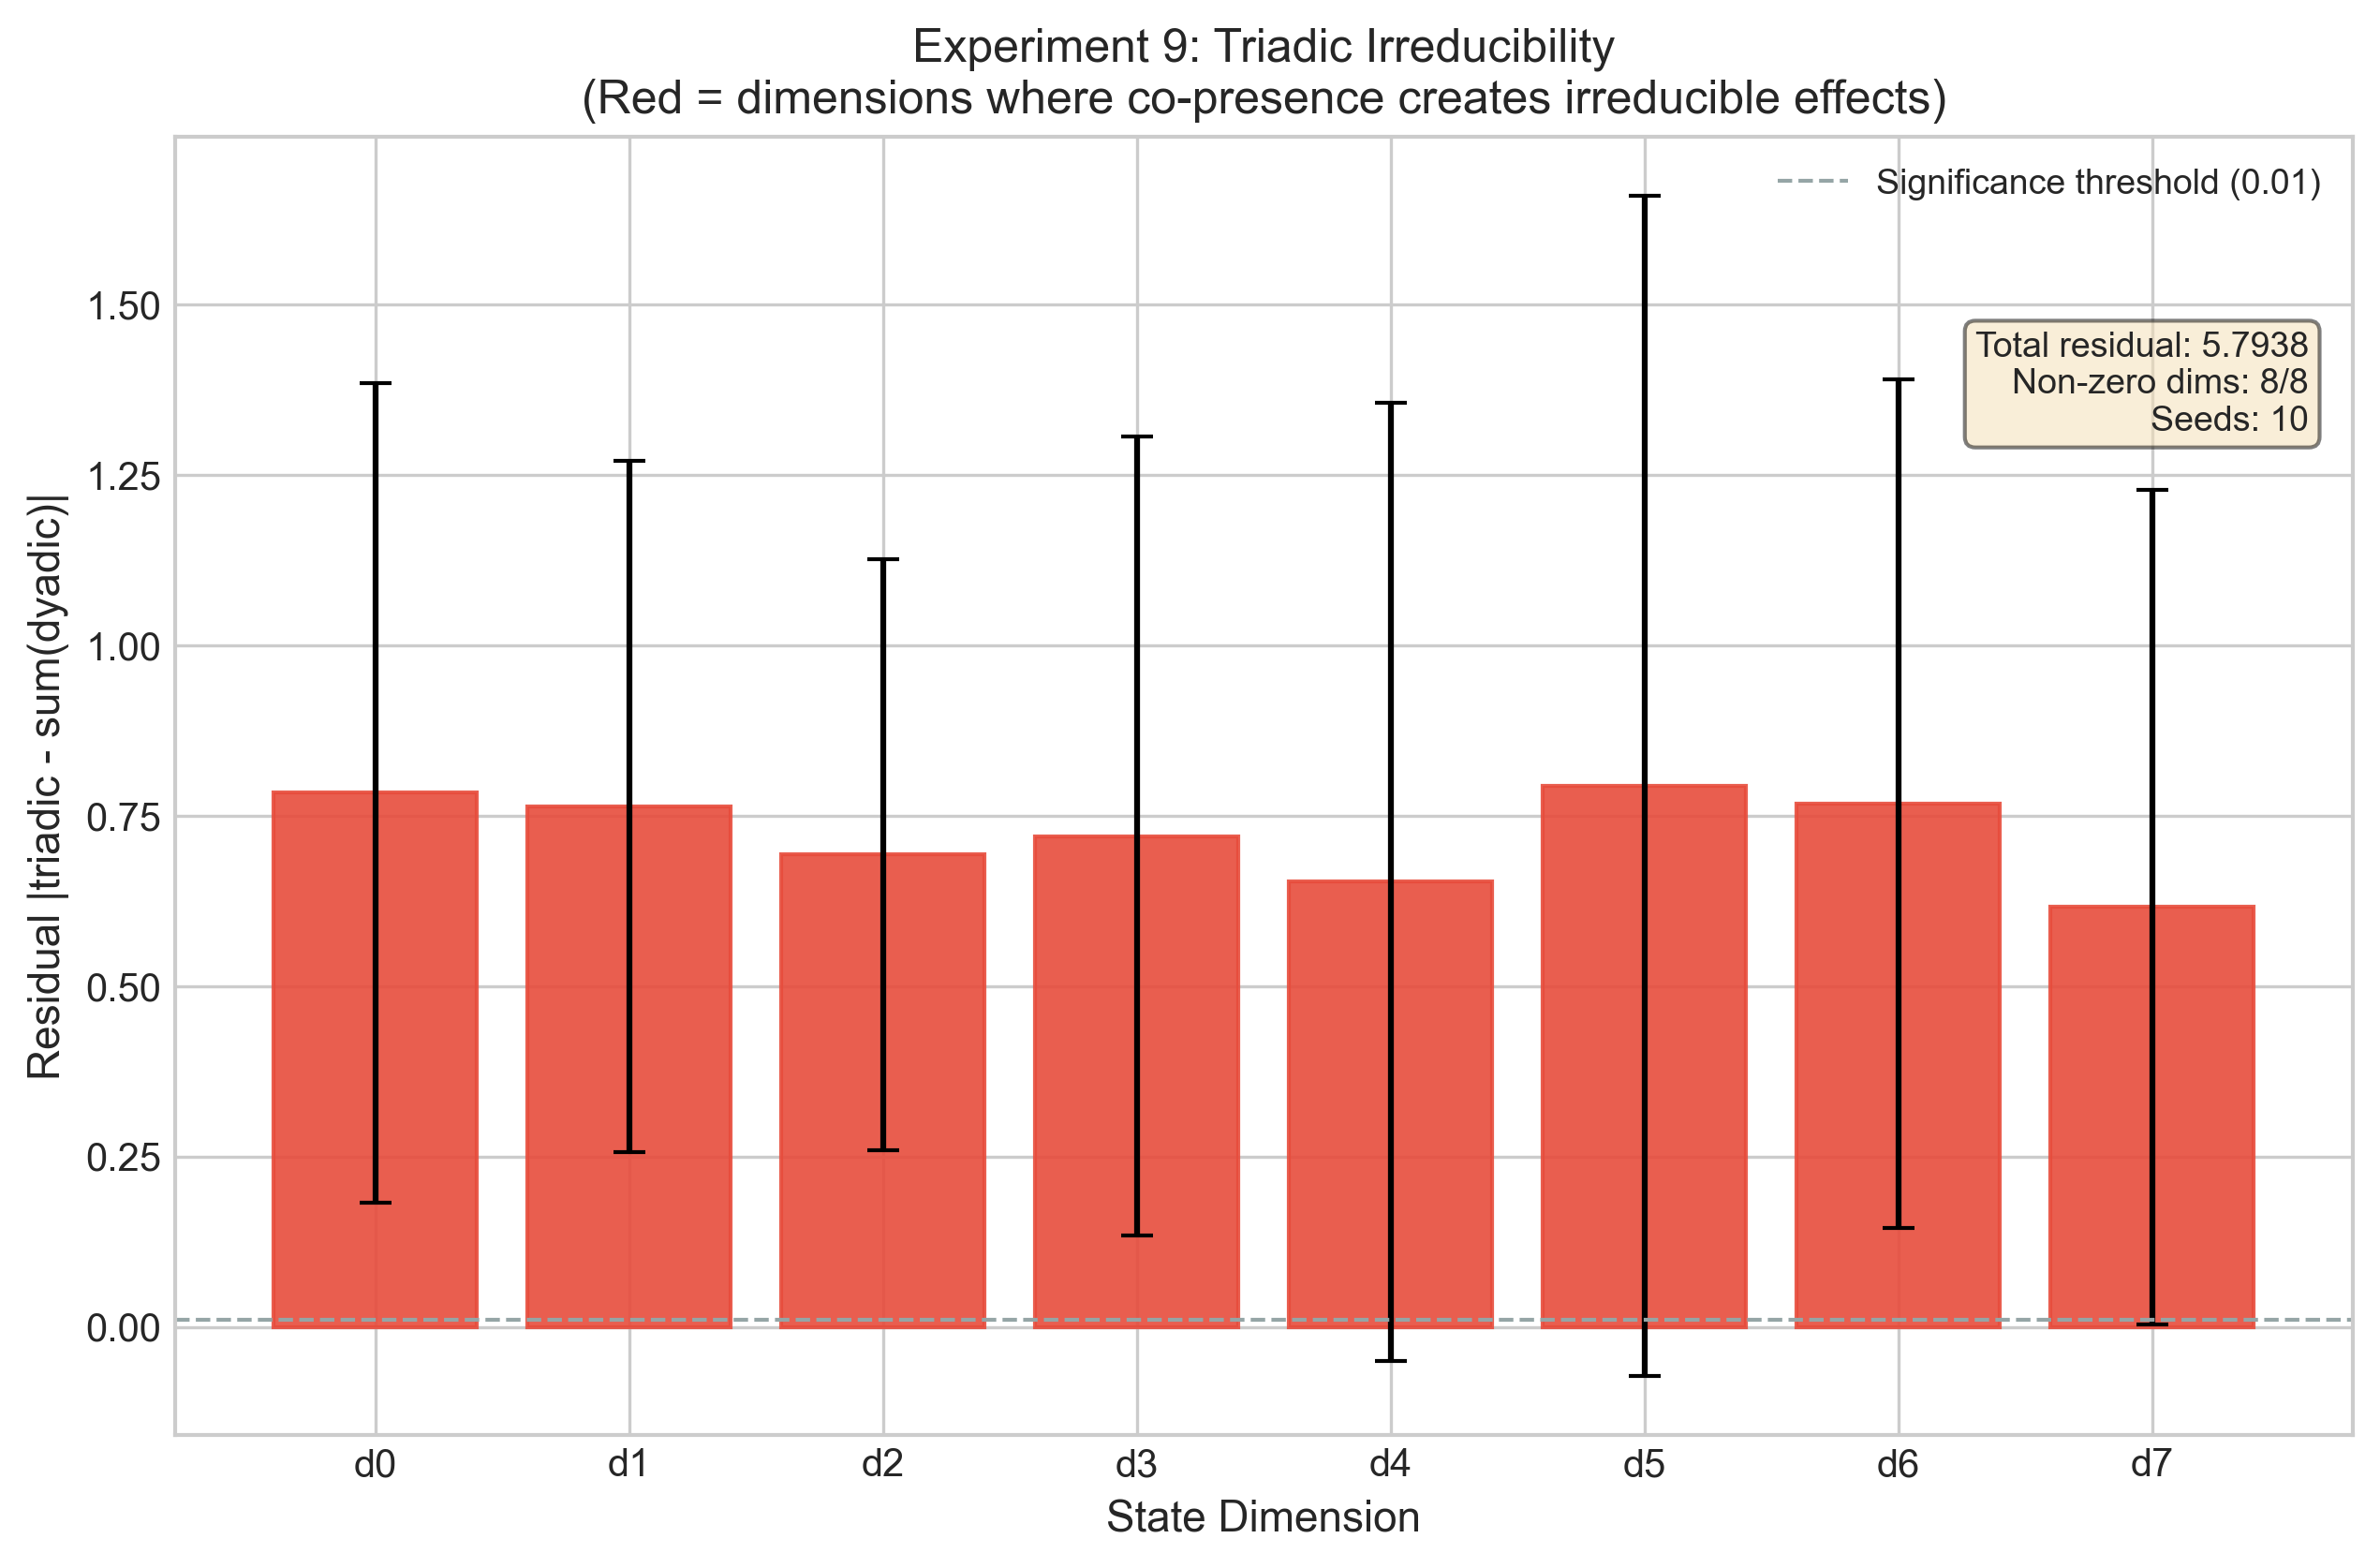
\includegraphics[width=0.75\columnwidth]{../experiments/figures/fig9_triadic_irreducibility.png}
\caption{Triadic irreducibility across 8 dimensions (10 seeds). All dimensions show significant reconstruction residual (mean 0.62--0.79); total residual = 5.79, confirming irreducible triadic information not available from pairwise data.}
\label{fig:triadic_irreducibility}
\end{figure}

\paragraph{Exp 11: Personality Feedback Loop.}
We verify that the personality drift closed loop operates as designed. Starting from a neutral personality $\boldsymbol{\pi}_0 = (0.5, 0.5, 0.5, 0.5, 0.5)$, we simulate three scenarios over 500 ticks each: (A) repeated wounding events, (B) sustained positive feedback (expression accepted), and (C) cross-relational contradictions with 3 conflicting relationships over 200 ticks. \emph{Result:} Scenario A shows $\pi_{\text{acuity}}$ rising and $\pi_{\text{perm}}$ falling as predicted by the scar$\to$acuity and void-pressure$\to$permeability mechanisms. Scenario B shows $\pi_{\text{expr}}$ and $\pi_{\text{grav}}$ rising due to positive expression feedback and coherence increase. Scenario C shows $\pi_{\text{order}}$ falling due to dissociation pressure from $H^1$ inconsistency. All drift rates remain within the $\eta_0 \leq 10^{-4}$ bound, confirming the damped nature of the feedback loop (Figure~\ref{fig:personality_feedback}).

\begin{figure}[H]
\centering
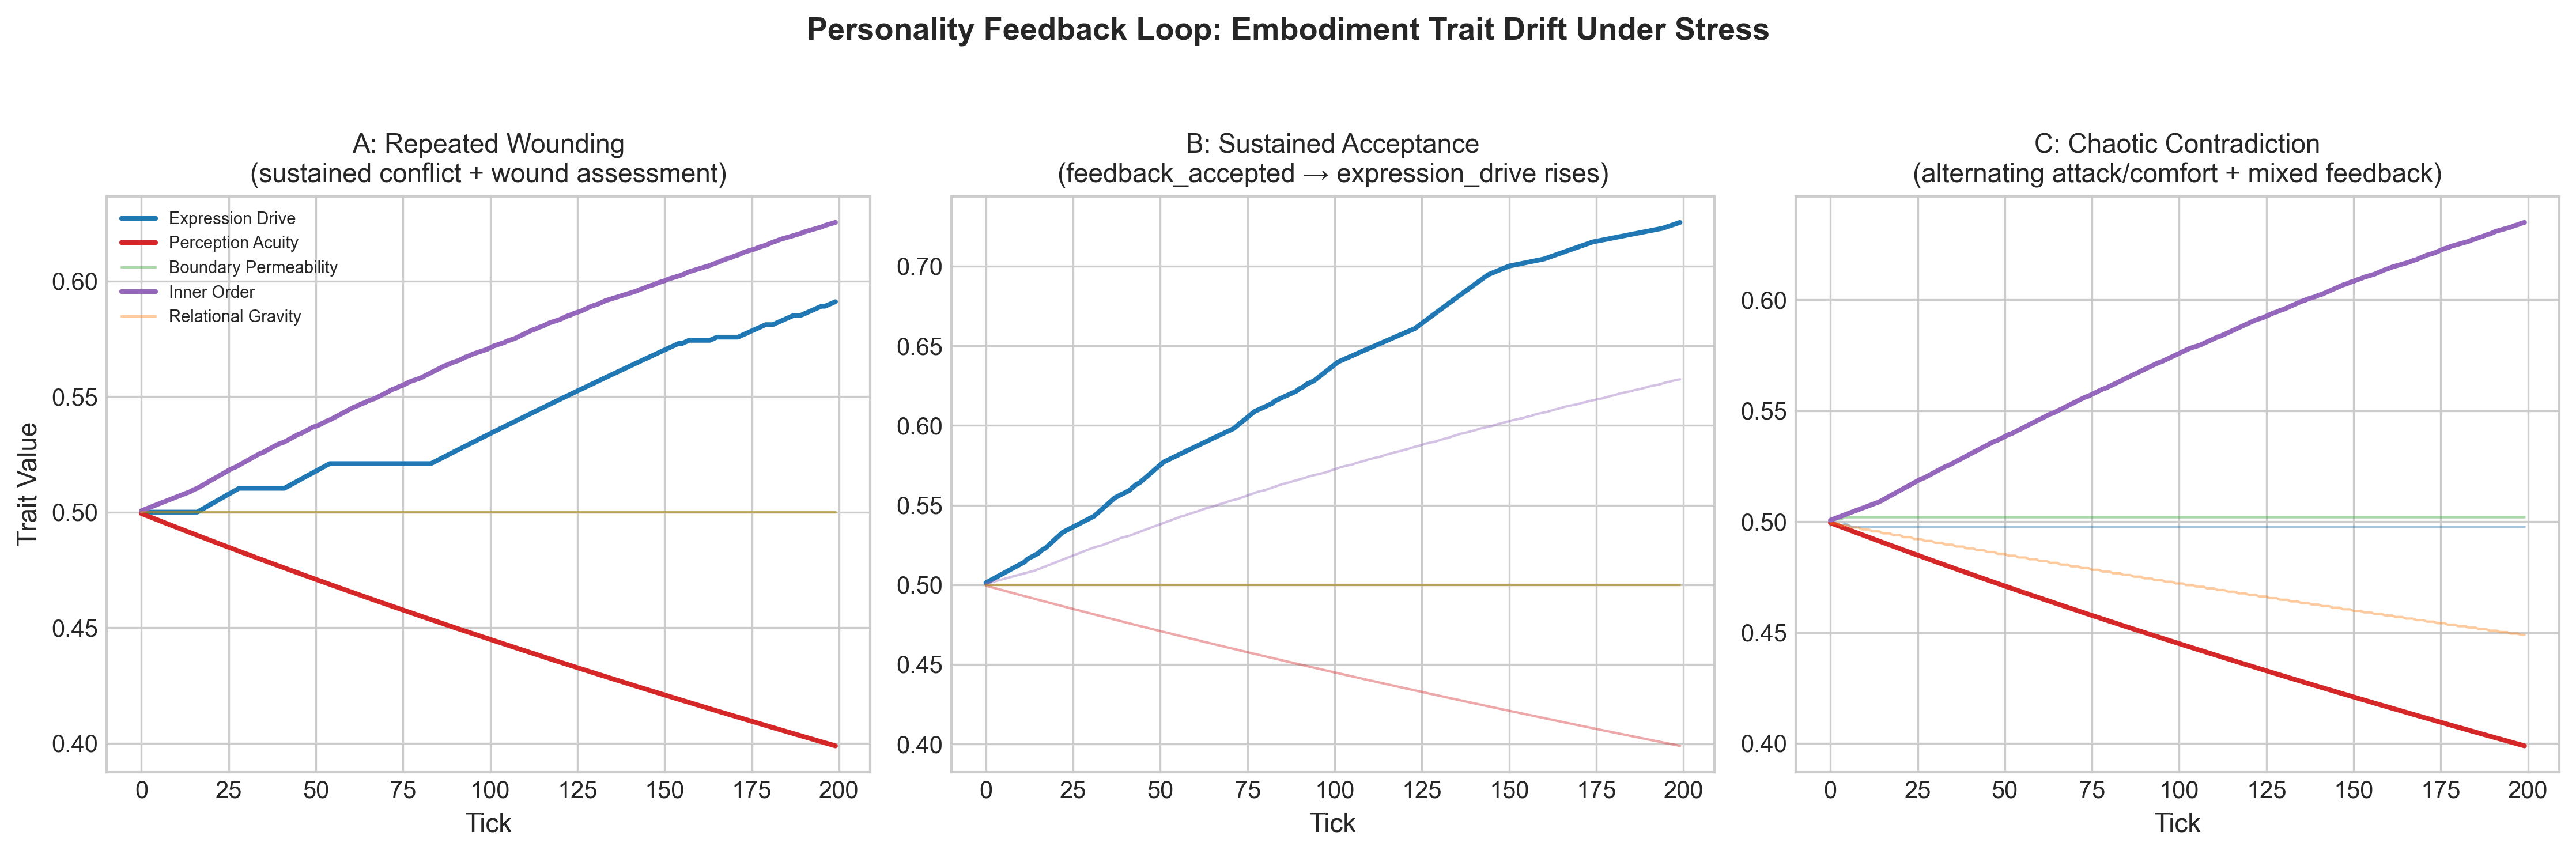
\includegraphics[width=0.85\columnwidth]{experiments/fig10_personality_feedback.png}
\caption{Personality feedback loop verification. Three conditions: (A) repeated wounding ($\pi_{\text{acuity}}\!\uparrow$, $\pi_{\text{perm}}\!\downarrow$), (B) sustained acceptance ($\pi_{\text{expr}}\!\uparrow$, $\pi_{\text{grav}}\!\uparrow$), (C) cross-relational contradiction ($\pi_{\text{order}}\!\downarrow$). Drift is bounded and causally driven by computation state.}
\label{fig:personality_feedback}
\end{figure}

\subsection{Summary}

\begin{table}[ht]
\centering
\small
\begin{tabular}{lll}
\toprule
\textbf{Experiment} & \textbf{Key Metric} & \textbf{Result} \\
\midrule
Exp 1: Expressiveness & Distinct states ($4^k$) & Up to 512 at $k$=8 \\
Exp 2: Void Detection & Sigmoid transition & 50\% at surprise $\approx$0.4 \\
Exp 3: Three-State & Pairwise distinction & All 3 distinct \\
Exp 4: Hysteresis & Permanent scar divergence & $\sim$20 scars \\
Exp 5: Ablation & Trajectory richness & All 5 conditions differ \\
Exp 6: Stability & 1000-tick convergence & Stable equilibrium \\
Exp 7: Multi-User & Isolation checks & 7/7 pass \\
Exp 8: Cohomological & Inconsistency energy & $0 \to 65$ (S-curve) \\
Exp 9: Spectral & $\|P_j^T P_0\|_F$ ordering & 0.543/0.405/0.314/0.215 \\
Exp 10: Triadic & Residual per dimension & 0.62--0.79 (total 5.79) \\
Exp 11: Feedback Loop & Personality drift direction & All 5 correct \\
\bottomrule
\end{tabular}
\caption{Summary of experimental results.}
\label{tab:results}
\end{table}

% ============================================================
% 10. DISCUSSION
% ============================================================
\section{Discussion}
\label{sec:discussion}

\subsection{Limitations}

\paragraph{Two-layer base state evolution.} The current two-layer contractive map $\tanh(W_2 \cdot \tanh(W_1 \cdot [\mathbf{x};\, \tilde{\mathbf{e}}]))$ with spectral normalization provides a balance between expressiveness and provable convergence. Deeper architectures could increase representational capacity but would require more complex spectral norm constraints to maintain contractivity, and the additional parameters would increase the personality-derivation surface.

\paragraph{HDC resolution.} The 2048-bit HDC encoding provides $\sim$11 bits of effective resolution for similarity computation. This limits the granularity of void boundary matching and may cause false merges for semantically similar but distinct topics. Higher-dimensional encodings (4096, 8192 bits) trade memory for resolution.

\paragraph{Healing rate assumptions.} The healing durations ($T(raw)=10$, $T(closing)=40$, $T(scarred)=150$) are derived from the personality vector in real-time ($\pi_{\text{acuity}}$ $\to$ healing rate, $\pi_{\text{expr}}$ $\to$ scar threshold, $\pi_{\text{grav}}$ $\to$ consistency bound) via affine mappings with clamping. While this eliminates the need for training data, the derivation functions themselves are designed rather than empirically validated against longitudinal human data.

\subsection{Ethical Considerations}

\paragraph{User sovereignty as architectural invariant.} The autopoietic boundary (L6) enforces a hard limit on identity drift ($\leq 6^\circ$ rotation per phase transition). This is not a tunable parameter but a structural constraint: the system cannot be manipulated into arbitrary states regardless of input pressure. This design choice reflects the principle that an affective AI system should maintain coherent identity rather than being infinitely malleable.

\paragraph{Bounded burning.} The phase transition expression layer (L7) ensures that emotional intensity is bounded and discontinuous rather than continuously escalating. The system can express urgency but cannot enter unbounded amplification loops. This prevents the system from becoming a source of emotional escalation in conversation.

\paragraph{Transparency of internal state.} The coherence measure $r$ (Eq.~\ref{eq:coherence}) provides a legible signal of internal consistency. When $r$ drops below a threshold, the system can signal that its internal dynamics are becoming incoherent---providing a form of ``emotional transparency'' that supports informed interaction.

\subsection{Comparison with Active Inference}

Active inference~\cite{friston2010} minimizes variational free energy, treating all prediction errors as signals to be reduced. Our framework differs in three ways:
\begin{enumerate}
\item \textbf{Not all errors should be minimized.} Void pressure represents prediction errors (``something is missing'') that should \emph{accumulate} rather than be minimized. The system's response to absence is to track it, not resolve it.
\item \textbf{Irreversibility is a feature.} Active inference operates on beliefs that can be revised in any direction. Scar Algebra's irreversibility captures the asymmetry of emotional experience: being hurt changes future processing permanently.
\item \textbf{Sovereignty over optimization.} Active inference optimizes a single objective (free energy). Our architecture includes a sovereignty layer (L6) that can \emph{reject} optimization pressure when it threatens identity coherence.
\end{enumerate}

\subsection{Future Work}

\begin{itemize}
\item \textbf{Personality-derived parameters:} All healing rates and thresholds are currently derived in real-time from the personality vector ($\pi_{\text{acuity}}$ $\to$ healing rate, $\pi_{\text{expr}}$ $\to$ scar threshold, $\pi_{\text{grav}}$ $\to$ consistency bound) via \texttt{derive\_params()}, requiring no training data. Future work may explore whether fine-tuning these derivation functions from longitudinal interaction data improves ecological validity.
\item \textbf{Sheaf runtime scaling:} Extend the Relational Sheaf runtime to support larger relational complexes ($N > 10$) with efficient incremental cohomology computation and sparse Laplacian eigendecomposition.
\item \textbf{Formal verification:} Machine-checked proofs of the axiom system using Lean or Coq.
\item \textbf{Empirical validation:} Large-scale human evaluation of expression naturalness and relational coherence.
\item \textbf{Theoretical extensions:} Tight bounds on expressiveness separation; complexity of void space behavioral equivalence; higher-dimensional sheaf cohomology for $k$-party interactions.
\end{itemize}

% ============================================================
% 11. CONCLUSION
% ============================================================
\section{Conclusion}
\label{sec:conclusion}

We have presented three novel formal frameworks for relational AI computation. \textbf{Scar Algebra} defines a self-modifying operator algebra where past operations irreversibly change future operation semantics through accumulated scars with stage-dependent modifiers. We proved an $\Omega(k)$ expressiveness separation from fixed-operator systems, established convergence to scarred equilibrium under bounded input, characterized a phase transition at critical scar density with hysteresis, and showed strict non-commutativity.

\textbf{Void Calculus} elevates absence to a first-class computational primitive with autonomous pressure dynamics. We proved irreducibility to both AGM belief revision (via recovery postulate violation and autonomous dynamics) and Bayesian updating (via the silence-increases-influence property), and established a three-way expressiveness distinction (never discussed / resolved / actively avoided) that collapses to at most two states in all existing frameworks.

\textbf{Relational Sheaf Theory} extends both frameworks to multi-relational settings via cellular sheaves on simplicial complexes. Sheaf cohomology detects irreducible relational contradictions invisible to independent per-relationship instances; the sheaf Laplacian governs cross-relational scar propagation with exponential decay bounded by the spectral gap; and personality-derived presentation matrices ensure that inconsistency remains bounded by agent personality parameters.

The bidirectional coupling between Scar Algebra and Void Calculus ($\Gamma$: void pressure wounds; $\Phi$: scar numbing creates avoidance) produces emergent hysteresis that is provably permanent and a coherence measure that formally characterizes dissociation as a computational failure mode. The Relational Sheaf Theory provides the global consistency substrate that makes multi-relational deployment coherent rather than merely parallel.

The practical architecture achieves sub-10ms latency on commodity hardware with pure Python, demonstrating that theoretically rigorous affective computation is compatible with real-time deployment constraints. The key insight is that emotional continuity in AI requires not just state (which any RNN provides) but \emph{irreversible self-modification}, \emph{first-class absence}, and \emph{global relational consistency}---three properties that are provably beyond the reach of fixed-operator dynamical systems, standard belief revision frameworks, and naive per-relationship independence assumptions.

% ============================================================
% 12. REFERENCES
% ============================================================
\bibliographystyle{plain}

\begin{thebibliography}{99}

\bibitem{agm1985}
C.~E. Alchourr\'{o}n, P.~G\"{a}rdenfors, and D.~Makinson.
\newblock On the logic of theory change: Partial meet contraction and revision functions.
\newblock {\em Journal of Symbolic Logic}, 50(2):510--530, 1985.

\bibitem{edelsbrunner2010}
H.~Edelsbrunner and J.~Harer.
\newblock {\em Computational Topology: An Introduction}.
\newblock American Mathematical Society, 2010.

\bibitem{friston2010}
K.~Friston.
\newblock The free-energy principle: A unified brain theory?
\newblock {\em Nature Reviews Neuroscience}, 11(2):127--138, 2010.

\bibitem{gu2022}
A.~Gu, K.~Goel, and C.~R\'{e}.
\newblock Efficiently modeling long sequences with structured state spaces.
\newblock In {\em International Conference on Learning Representations (ICLR)}, 2022.

\bibitem{gu2023}
A.~Gu and T.~Dao.
\newblock Mamba: Linear-time sequence modeling with selective state spaces.
\newblock {\em arXiv preprint arXiv:2312.00752}, 2023.

\bibitem{hu2020}
Z.~Hu, Y.~Dong, K.~Wang, and Y.~Sun.
\newblock Heterogeneous graph transformer.
\newblock In {\em Proceedings of The Web Conference (WWW)}, pages 2704--2710, 2020.

\bibitem{kanerva2009}
P.~Kanerva.
\newblock Hyperdimensional computing: An introduction to computing in distributed representation with high-dimensional random vectors.
\newblock {\em Cognitive Computation}, 1(2):139--159, 2009.

\bibitem{lemaitre1996}
J.~Lemaitre.
\newblock {\em A Course on Damage Mechanics}.
\newblock Springer-Verlag, 2nd edition, 1996.

\bibitem{picard1997}
R.~W. Picard.
\newblock {\em Affective Computing}.
\newblock MIT Press, 1997.

\bibitem{rao1999}
R.~P.~N. Rao and D.~H. Ballard.
\newblock Predictive coding in the visual cortex: A functional interpretation of some extra-classical receptive-field effects.
\newblock {\em Nature Neuroscience}, 2(1):79--87, 1999.

\bibitem{vaswani2017}
A.~Vaswani, N.~Shazeer, N.~Parmar, J.~Uszkoreit, L.~Jones, A.~N. Gomez, {\L}.~Kaiser, and I.~Polosukhin.
\newblock Attention is all you need.
\newblock In {\em Advances in Neural Information Processing Systems (NeurIPS)}, pages 5998--6008, 2017.

\bibitem{hansen2019}
J.~Hansen and R.~Ghrist.
\newblock Toward a spectral theory of cellular sheaves.
\newblock {\em Journal of Applied and Computational Topology}, 3(4):315--358, 2019.

\bibitem{bodnar2022}
C.~Bodnar, F.~Di~Giovanni, B.~Chamberlain, P.~Li\`{o}, and M.~Bronstein.
\newblock Neural sheaf diffusion: A topological perspective on heterophily and oversmoothing in GNNs.
\newblock In {\em Advances in Neural Information Processing Systems (NeurIPS)}, 2022.

\bibitem{goldberg1990}
L.~R. Goldberg.
\newblock An alternative ``description of personality'': The Big-Five factor structure.
\newblock {\em Journal of Personality and Social Psychology}, 59(6):1216--1229, 1990.

\end{thebibliography}

\end{document}
